% =============================================================================
%  Machine Learning for Petroleum Engineers Using Python
%  Módulo 5 · Clase 2: El pozo avisa antes de romperse --- detección en
%  señales de sensores (3W Dataset, Petrobras)
%  SLB Ecuador | UDLA
%
%  Compilar: pdflatex -shell-escape presentacion.tex (x2 para refs)
% =============================================================================
\documentclass[aspectratio=169, 11pt]{beamer}

% ── Codificación y lenguaje ──────────────────────────────────────────────────
\usepackage[T1]{fontenc}
\usepackage[utf8]{inputenc}
\usepackage[spanish,es-noshorthands]{babel}

% ── Fuentes ──────────────────────────────────────────────────────────────────
\usepackage{FiraSans}
\usepackage{FiraMono}
\renewcommand{\familydefault}{\sfdefault}

% ── Gráficos y diagramas ────────────────────────────────────────────────────
\usepackage{graphicx}
\usepackage{tikz}
\usetikzlibrary{arrows.meta, positioning, shapes.geometric, calc, fit, decorations.pathreplacing}
\usepackage{fontawesome5}

% ── Código fuente ────────────────────────────────────────────────────────────
\usepackage{minted}
\usepackage{tcolorbox}
\tcbuselibrary{minted, skins, breakable}

% ── Tablas y utilidades ──────────────────────────────────────────────────────
\usepackage{amsmath}
\usepackage{colortbl}
\usepackage{booktabs}
\usepackage{multicol}
\usepackage{hyperref}
\usepackage{calc}

% =============================================================================
%  PALETA DE COLORES (rojo UDLA + variantes)
% =============================================================================
\definecolor{arcaRed}{HTML}{C82B40}
\definecolor{arcaDark}{HTML}{6B1525}
\definecolor{udlaCrimson}{HTML}{A31545}
\definecolor{arcaGray}{HTML}{F5F5F5}
\definecolor{arcaLightGray}{HTML}{EBEBEB}
\definecolor{textDark}{HTML}{2D2D2D}
\definecolor{textMuted}{HTML}{6B7280}
\definecolor{codeGreen}{HTML}{16A34A}
\definecolor{codeBlue}{HTML}{2563EB}
\definecolor{codeOrange}{HTML}{EA580C}
\definecolor{slbBlue}{HTML}{0014DC}
\definecolor{terminalBg}{HTML}{0F172A}
\definecolor{terminalGreen}{HTML}{86EFAC}
\definecolor{terminalMuted}{HTML}{94A3B8}
\definecolor{codeBg}{HTML}{FAFAFA}

% =============================================================================
%  CONFIGURACIÓN DEL TEMA BEAMER
% =============================================================================
\usetheme{default}
\usecolortheme{default}

\setbeamertemplate{navigation symbols}{}
\setbeamertemplate{footline}{}
\setbeamertemplate{headline}{}

\setbeamercolor{normal text}{fg=textDark}
\setbeamercolor{frametitle}{fg=arcaRed, bg=white}
\setbeamercolor{title}{fg=white}
\setbeamercolor{subtitle}{fg=white!85}
\setbeamercolor{author}{fg=white!80}
\setbeamercolor{date}{fg=white!70}
\setbeamercolor{item}{fg=arcaRed}
\setbeamercolor{subitem}{fg=arcaDark}
\setbeamercolor{block title}{fg=white, bg=arcaRed}
\setbeamercolor{block body}{fg=textDark, bg=arcaGray}
\setbeamercolor{block title alerted}{fg=white, bg=codeOrange}
\setbeamercolor{block body alerted}{fg=textDark, bg=arcaGray}
\setbeamercolor{block title example}{fg=white, bg=codeGreen}
\setbeamercolor{block body example}{fg=textDark, bg=arcaGray}
\setbeamercolor{section in toc}{fg=arcaDark}

\setbeamerfont{frametitle}{size=\Large, series=\bfseries}
\setbeamerfont{title}{size=\huge, series=\bfseries}
\setbeamerfont{subtitle}{size=\large}
\setbeamerfont{author}{size=\normalsize}
\setbeamerfont{date}{size=\small}
\setbeamerfont{block title}{size=\normalsize, series=\bfseries}
\setbeamerfont{footnote}{size=\tiny}

\setbeamertemplate{itemize item}{\scriptsize\raise1.5pt\hbox{\color{arcaRed}$\blacktriangleright$}}
\setbeamertemplate{itemize subitem}{\scriptsize\raise1pt\hbox{\color{arcaDark}$\bullet$}}
\setbeamertemplate{enumerate items}[default]
\setbeamercolor{enumerate item}{fg=arcaRed}

% =============================================================================
%  HEADER
% =============================================================================
\setbeamertemplate{headline}{%
  \begin{tikzpicture}[remember picture, overlay]
    \fill[arcaDark] (current page.north west) rectangle
      ([yshift=-0.7cm]current page.north east);
    \node[anchor=west, inner sep=0pt] at
      ([xshift=0.6cm, yshift=-0.35cm]current page.north west)
      {
\includegraphics[height=0.45cm]{../logo_udla_white.png}};
    \node[anchor=east, inner sep=0pt] at
      ([xshift=-0.6cm, yshift=-0.35cm]current page.north east)
      {
\includegraphics[height=0.42cm]{../SLB_white.png}};
  \end{tikzpicture}%
  \vspace{0.7cm}%
}

% =============================================================================
%  FOOTER
% =============================================================================
\setbeamertemplate{footline}{%
  \begin{tikzpicture}[remember picture, overlay]
    \draw[arcaLightGray, line width=0.4pt]
      ([yshift=0.55cm, xshift=0.6cm]current page.south west) --
      ([yshift=0.55cm, xshift=-0.6cm]current page.south east);
    \node[anchor=south, font=\tiny\color{textMuted}] at
      ([yshift=0.15cm]current page.south)
      {Machine Learning for Petroleum Engineers Using Python \(\cdot\) SLB Ecuador};
    \node[anchor=south east, font=\scriptsize\bfseries\color{arcaRed}] at
      ([xshift=-0.6cm, yshift=0.15cm]current page.south east)
      {\insertframenumber};
  \end{tikzpicture}%
}

% =============================================================================
%  FRAMETITLE personalizado con línea roja
% =============================================================================
\setbeamertemplate{frametitle}{%
  \vspace{0.25cm}%
  \usebeamerfont{frametitle}\usebeamercolor[fg]{frametitle}\insertframetitle%
  \par\vspace{2pt}%
  \begin{tikzpicture}
    \fill[arcaRed] (0,0) rectangle (3cm, 1.5pt);
    \fill[arcaLightGray] (3cm,0) rectangle (\textwidth, 0.5pt);
  \end{tikzpicture}%
  \vspace{0.1cm}%
}

% =============================================================================
%  ESTILO DE BLOQUES DE CÓDIGO (minted + tcolorbox)
% =============================================================================
\newtcblisting{pyblock}[1][]{%
  listing engine=minted,
  minted language=python,
  minted style=xcode,
  minted options={
    fontsize=\small,
    linenos=false,
    breaklines=true,
    python3=true
  },
  enhanced,
  colback=codeBg,
  colframe=arcaRed,
  left=8pt,
  right=6pt,
  top=5pt,
  bottom=5pt,
  boxrule=0pt,
  leftrule=3pt,
  arc=3pt,
  listing only,
  title={\hspace{-2pt}\faPython\hspace{5pt}Python},
  fonttitle=\scriptsize\bfseries,
  colbacktitle=arcaRed,
  coltitle=white,
  attach boxed title to top left={xshift=8pt, yshift=-7pt},
  boxed title style={
    arc=2pt, boxrule=0pt,
    top=1.5pt, bottom=1.5pt, left=6pt, right=6pt
  },
  drop fuzzy shadow=black!12,
  #1
}

\newtcblisting{outputblock}[1][]{%
  listing engine=minted,
  minted language=text,
  minted style=bw,
  minted options={
    fontsize=\small,
    breaklines=true,
    formatcom=\color{terminalGreen}
  },
  enhanced,
  colback=terminalBg,
  colframe=terminalBg,
  coltext=terminalGreen,
  left=10pt, right=6pt, top=5pt, bottom=5pt,
  boxrule=0pt,
  arc=3pt,
  listing only,
  title={\hspace{-2pt}\faTerminal\hspace{5pt}Output},
  fonttitle=\scriptsize\bfseries,
  colbacktitle=terminalGreen!85!black,
  coltitle=terminalBg,
  attach boxed title to top left={xshift=8pt, yshift=-7pt},
  boxed title style={
    arc=2pt, boxrule=0pt,
    top=1.5pt, bottom=1.5pt, left=6pt, right=6pt
  },
  #1
}

% =============================================================================
%  SECTION DIVIDERS
% =============================================================================
\newcommand{\sectionframe}[2]{%
  \begingroup
    \setbeamertemplate{headline}{}
    \setbeamertemplate{footline}{}
    \setbeamertemplate{navigation symbols}{}
    \begin{frame}[plain, noframenumbering]
      \begin{tikzpicture}[remember picture, overlay]
        \fill[arcaRed] (current page.south west) rectangle (current page.north east);
        \node[anchor=center, text=white, font=\Huge\bfseries, text width=15cm,
              align=center] at ([yshift=0.5cm]current page.center)
              {\hyphenpenalty=10000\exhyphenpenalty=10000 #1};
        \node[anchor=center, text=white!80, font=\large, text width=10cm,
              align=center] at ([yshift=-0.8cm]current page.center) {#2};
      \end{tikzpicture}
    \end{frame}
  \endgroup
}

% =============================================================================
%  METADATOS
% =============================================================================
\title{Machine Learning for Petroleum Engineers\\Using Python}
\subtitle{Módulo 3 · Clase 5: SVM, Pipelines y Validación Honesta}
\author{Carlos Enrique Mosquera Trujillo}
\date{2026}

% =============================================================================
%  DOCUMENTO
% =============================================================================
% =============================================================================
%  DOCUMENTO
% =============================================================================
\begin{document}
% ── PORTADA ──────────────────────────────────────────────────────────────────
{
\setbeamertemplate{headline}{}
\setbeamertemplate{footline}{}
\begin{frame}[plain, noframenumbering]
  \begin{tikzpicture}[remember picture, overlay]
    \fill[white] (current page.south west) rectangle (current page.north east);
    \fill[arcaRed] (current page.north west) rectangle ([yshift=-0.35cm]current page.north east);
    \fill[arcaDark] (current page.south west) rectangle ([yshift=0.35cm]current page.south east);
    \fill[arcaRed]
      ([xshift=1.1cm, yshift=-0.35cm]current page.north west) rectangle
      ([xshift=1.15cm, yshift=0.35cm]current page.south west);
    \node[anchor=north west, inner sep=0pt] at
      ([xshift=1.8cm, yshift=-1.2cm]current page.north west)
      {
\includegraphics[height=1.6cm]{../logo_udla.png}};
    \node[anchor=north east, inner sep=0pt] at
      ([xshift=-1.5cm, yshift=-1.2cm]current page.north east)
      {
\includegraphics[height=1.5cm]{../SLB.png}};
    \node[anchor=center, text=arcaDark, text width=14.5cm, align=center] at
      ([yshift=0.95cm]current page.center) {
        {\LARGE\bfseries Machine Learning for Petroleum Engineers}\\[8pt]
        {\LARGE\bfseries Using Python}
      };
    \fill[arcaRed]
      ([yshift=-0.35cm, xshift=-3.2cm]current page.center) rectangle
      ([yshift=-0.28cm, xshift=3.2cm]current page.center);
    \node[anchor=center, text=arcaRed, font=\large, text width=13cm, align=center] at
      ([yshift=-1.3cm]current page.center) {
        Módulo 5 · Clase 2\\[3pt]
        El Pozo Avisa Antes de Romperse --- Detectar en Señales de Sensores
      };
    \node[anchor=center, text=textMuted, font=\normalsize] at
      ([yshift=-2.5cm]current page.center) {
        {\color{arcaRed}\faUser}\hspace{6pt}Carlos Enrique Mosquera Trujillo
        \hspace{16pt}
        {\color{arcaRed}\faIndustry}\hspace{4pt}SLB Ecuador
      };
  \end{tikzpicture}
\end{frame}
}

% ── RECAP + RUTA ─────────────────────────────────────────────────────────────
\begin{frame}[shrink=8]{Dónde Estamos: la Segunda Clase del Módulo 5}
  \vspace{-4pt}
  \begin{columns}[T]
    \begin{column}{0.48\textwidth}
      {\small\color{arcaDark}\bfseries\faCheckCircle\hspace{5pt}Ya saben:}
      \vspace{4pt}
      {\footnotesize\color{textMuted}
      \begin{itemize}\setlength{\itemsep}{3pt}
        \item[{\color{codeGreen}\scriptsize\faCheck}]
          Que un dato con \textbf{orden en el tiempo} no se puede barajar (M5·C1)
        \item[{\color{codeGreen}\scriptsize\faCheck}]
          Predecir una \textbf{etiqueta} con \textbf{Random Forest} (M3·C3)
        \item[{\color{codeGreen}\scriptsize\faCheck}]
          Que hay que \textbf{validar dejando pozos completos por fuera} (M3·C5)
        \item[{\color{codeGreen}\scriptsize\faCheck}]
          Que el error se mide en \textbf{dólares}, no en puntos
      \end{itemize}
      }
      \vspace{5pt}
      {\scriptsize\color{textMuted}\itshape
        Nada de esto se da por sabido: cada pieza que usemos hoy
        se vuelve a explicar desde cero cuando aparece.}
    \end{column}
    \begin{column}{0.48\textwidth}
      {\small\color{arcaDark}\bfseries\faForward\hspace{5pt}Hoy:}
      \vspace{4pt}
      {\footnotesize\color{textMuted}
      \begin{itemize}\setlength{\itemsep}{3pt}
        \item[{\color{arcaRed}\scriptsize\faArrowRight}]
          Una pregunta nueva: ya no \emph{cuánto}, sino \textbf{cuándo y qué hago}
        \item[{\color{arcaRed}\scriptsize\faArrowRight}]
          Sensores reales de \textbf{pozos submarinos}, a una medición por segundo
        \item[{\color{arcaRed}\scriptsize\faArrowRight}]
          \textbf{Descomponer} una señal para convertirla en una tabla
        \item[{\color{arcaRed}\scriptsize\faStar}]
          Y una sorpresa: el salto grande \textbf{no lo da el modelo}
      \end{itemize}
      }
      \vspace{4pt}
      {\scriptsize\color{arcaDark}\itshape
        Cerramos con el marcador contra la alarma
        que hoy está instalada en la sala de control.}
    \end{column}
  \end{columns}
\end{frame}

% ── ANDRAGOGÍA ───────────────────────────────────────────────────────────────
\begin{frame}[shrink=6]{Ustedes Ya Hacen Esto}
  \vspace{-4pt}
  {\small\color{arcaDark}\bfseries
   Antes de que aparezca una sola fórmula: el trabajo de hoy ya lo saben hacer.}
  \vspace{8pt}
  \begin{columns}[T]
    \begin{column}{0.52\textwidth}
      \begin{tcolorbox}[colback=arcaGray, colframe=arcaRed, boxrule=0pt, leftrule=3pt,
        arc=3pt, left=6pt, right=6pt, top=5pt, bottom=5pt]
        {\scriptsize\color{arcaRed}\bfseries\faUserCog\hspace{4pt}SU PROBLEMA DIARIO}\\[4pt]
        {\scriptsize\color{textMuted}
         Un operador mira la pantalla del pozo y dice:
         \textit{«este pozo hoy está raro»}.\\[4pt]
         No calculó nada. Comparó lo que ve contra lo que ese pozo
         \textbf{suele} hacer, miró \textbf{varias} pantallas a la vez,
         y notó que la cosa \textbf{venía cambiando} hace rato.}
      \end{tcolorbox}
    \end{column}
    \begin{column}{0.44\textwidth}
      {\footnotesize\color{textMuted}
      Eso que hizo el operador tiene tres partes, y son exactamente
      las tres que vamos a programar hoy:
      \vspace{6pt}
      \begin{itemize}\setlength{\itemsep}{5pt}
        \item[{\color{arcaRed}\scriptsize\faArrowRight}]
          contra \textbf{lo que ese pozo suele hacer}
        \item[{\color{arcaRed}\scriptsize\faArrowRight}]
          mirando \textbf{varias señales juntas}
        \item[{\color{arcaRed}\scriptsize\faArrowRight}]
          atento a que \textbf{venía cambiando}
      \end{itemize}
      }
      \vspace{6pt}
      {\scriptsize\color{arcaDark}\itshape
        El modelo no va a ser más listo que el operador.
        Va a hacer lo mismo, en los 40 pozos, las 24 horas.}
    \end{column}
  \end{columns}
\end{frame}

% ── EL ENCARGO ───────────────────────────────────────────────────────────────
\begin{frame}[shrink=6]{El Encargo}
  \vspace{-4pt}
  \begin{tcolorbox}[colback=arcaGray, colframe=arcaDark, boxrule=0pt, leftrule=3pt,
    arc=3pt, left=8pt, right=8pt, top=6pt, bottom=6pt]
    {\small\color{arcaDark}\itshape
     Un pozo submarino a 1\,200 metros de profundidad. El choke de producción
     --- la válvula que regula cuánto sale --- se está \textbf{incrustando}: se
     le pegan sales por dentro y se va cerrando solo.\\[5pt]
     La sala de control tiene una alarma. Cuando suena, el pozo ya está en falla.\\[5pt]
     \textbf{La pregunta de hoy: ¿cuánto antes se puede saber?}}
  \end{tcolorbox}
  \vspace{6pt}
  \begin{columns}[T]
    \begin{column}{0.49\textwidth}
      {\small\color{arcaDark}\bfseries\faDollarSign\hspace{5pt}Por qué importa la anticipación:}
      \vspace{3pt}
      {\footnotesize\color{textMuted}
      \begin{itemize}\setlength{\itemsep}{3pt}
        \item[{\color{arcaRed}\scriptsize\faExclamationTriangle}]
          Si me entero \textbf{cuando ya falló}: el pozo se cierra sin avisar,
          y una intervención submarina necesita \textbf{barco}
        \item[{\color{codeGreen}\scriptsize\faCheck}]
          Si me entero \textbf{horas antes}: se abre el choke, se inyecta
          inhibidor, se programa la parada con el resto del campo
      \end{itemize}
      }
    \end{column}
    \begin{column}{0.49\textwidth}
      {\small\color{arcaDark}\bfseries\faClock\hspace{5pt}La unidad de la respuesta:}
      \vspace{3pt}
      {\footnotesize\color{textMuted}
      La respuesta de hoy \textbf{no es un porcentaje}. Son \textbf{minutos}.\\[5pt]
      Cada minuto que ganamos es un minuto en que alguien todavía puede
      hacer algo. Cuando el pozo ya falló, no hay nada que decidir:
      solo hay que pagar.}
      \vspace{5pt}
      {\scriptsize\color{arcaDark}\itshape
        Por eso, toda la clase, la métrica va a ser la misma:
        \textbf{¿cuántos minutos antes?}}
    \end{column}
  \end{columns}
\end{frame}

% ── ACOTAR EL PROBLEMA ───────────────────────────────────────────────────────
\begin{frame}[shrink=10]{Acotar el Problema (Regla de la Casa)}
  \vspace{-4pt}
  {\small\color{arcaDark}\bfseries
   Ninguna línea de código antes de llenar esta tabla. Ninguna. Nunca.}
  \vspace{8pt}
  {\footnotesize
  \renewcommand{\arraystretch}{1.35}
  \begin{tabular}{@{}p{3.4cm}p{11.2cm}@{}}
    \toprule
    {\color{arcaDark}\bfseries Pregunta de negocio} &
      ¿Cuántos minutos antes de la falla puedo avisarle al operador? \\
    {\color{arcaDark}\bfseries Lo que predigo} &
      Una etiqueta, en cada instante: \textbf{¿este pozo está entrando en falla, sí o no?} \\
    {\color{arcaDark}\bfseries Con qué} &
      Cinco sensores de fondo y de árbol submarino, una medición cada 30 segundos \\
    {\color{arcaDark}\bfseries Métrica de éxito} &
      Dos, juntas: \textbf{cuántos casos detecta} (de 10) y \textbf{a los cuántos minutos} \\
    \rowcolor{arcaGray}
    {\color{arcaDark}\bfseries Récord a batir} &
      {\color{arcaRed}\bfseries La alarma que hoy está instalada.} La medimos en un rato:
      hasta entonces, nadie sabe si es buena o mala \\
    \bottomrule
  \end{tabular}}
  \vspace{9pt}

  {\scriptsize\color{textMuted}\itshape
   Fíjense en la última fila. No arrancamos comparando contra cero:
   arrancamos comparando contra \textbf{lo que ya existe y ya funciona}.
   Un modelo que no le gana a lo instalado no se instala.}
\end{frame}

% ═════════════════════════════════════════════════════════════════════════════
\sectionframe{El Pozo y lo que Mide}{Qué es un choke, por qué se tapa, y qué es exactamente un archivo de sensores \\[6pt] \normalsize 12 -- 42 min}
% ═════════════════════════════════════════════════════════════════════════════

\begin{frame}[shrink=6]{Un Pozo que Nadie Puede Ir a Mirar}
  \vspace{-6pt}
  \begin{center}
    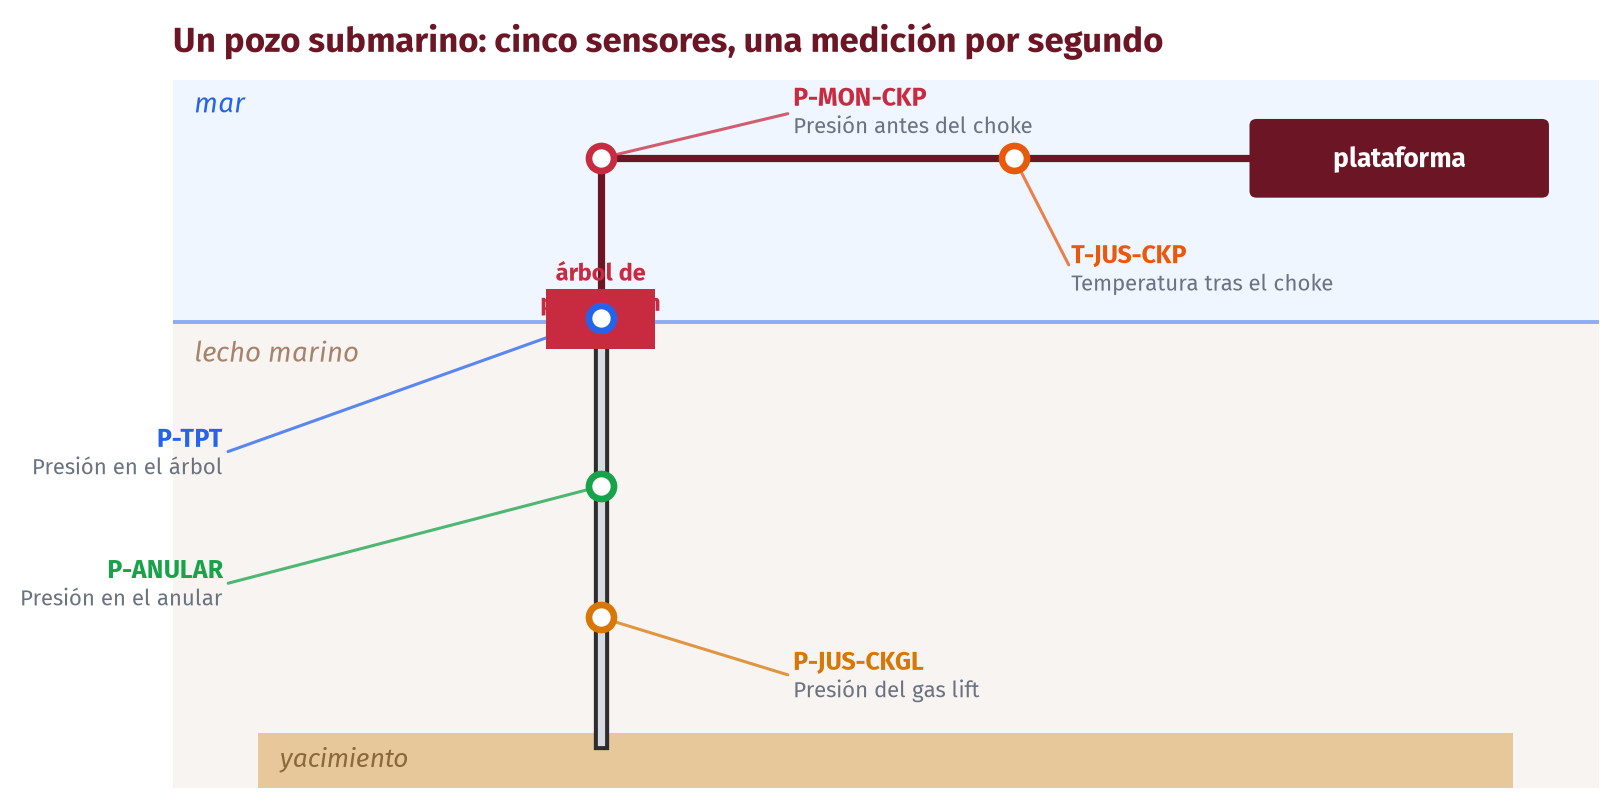
\includegraphics[height=0.60\textheight]{fig_pozo.png}
  \end{center}
  \vspace{-4pt}
  {\footnotesize\color{textMuted}
  \begin{itemize}\setlength{\itemsep}{2pt}
    \item[{\color{arcaRed}\scriptsize\faArrowRight}]
      El equipo está en el \textbf{lecho marino}. Nadie baja a mirarlo: para
      tocarlo hace falta un barco y una ventana de buen tiempo.
    \item[{\color{arcaRed}\scriptsize\faArrowRight}]
      Lo único que llega a superficie son \textbf{números}. Esos cinco.
  \end{itemize}}
\end{frame}

\begin{frame}[shrink=8]{¿Qué es un Choke? La Pieza de Toda la Clase}
  \vspace{-4pt}
  {\small\color{arcaDark}\bfseries
   Empecemos por acá, porque si esta pieza no queda clara, nada de lo que
   sigue tiene sentido.}
  \vspace{8pt}
  \begin{columns}[T]
    \begin{column}{0.49\textwidth}
      {\footnotesize\color{textMuted}
      El \textbf{choke} (o estrangulador) es una válvula con un agujero
      calibrado, puesta a la salida del pozo. Todo lo que el pozo produce
      pasa obligatoriamente por ese agujero.\\[6pt]
      Es, literalmente, \textbf{la boquilla de la manguera}: si la aprietan,
      sale menos agua y sale con más fuerza; si la abren, sale más y más
      floja.}
      \vspace{7pt}
      \begin{tcolorbox}[colback=arcaGray, colframe=arcaDark, boxrule=0pt, leftrule=3pt,
        arc=3pt, left=6pt, right=6pt, top=4pt, bottom=4pt]
        {\scriptsize\color{textMuted}
         Es la \textbf{única perilla} que el operador tiene para controlar
         cuánto produce un pozo submarino. Nada más se puede tocar desde
         arriba.}
      \end{tcolorbox}
    \end{column}
    \begin{column}{0.47\textwidth}
      {\small\color{arcaDark}\bfseries\faQuestion\hspace{5pt}¿Y por qué no se deja abierto?}
      \vspace{4pt}
      {\footnotesize\color{textMuted}
      Porque producir al máximo rompe cosas:
      \vspace{4pt}
      \begin{itemize}\setlength{\itemsep}{4pt}
        \item[{\color{arcaRed}\scriptsize\faArrowRight}]
          Si el pozo va muy rápido, \textbf{arrastra arena} y erosiona la
          tubería
        \item[{\color{arcaRed}\scriptsize\faArrowRight}]
          \textbf{Chupa agua} del acuífero antes de tiempo
        \item[{\color{arcaRed}\scriptsize\faArrowRight}]
          La planta de arriba tiene una \textbf{capacidad}, y no la puede pasar
      \end{itemize}}
      \vspace{6pt}
      {\scriptsize\color{arcaDark}\itshape
        Por eso el choke está siempre a medio abrir, en una posición
        que alguien eligió y anotó.}
    \end{column}
  \end{columns}
\end{frame}

\begin{frame}[shrink=6]{Lo que le Hace el Choke al Fluido}
  \vspace{-8pt}
  \begin{center}
    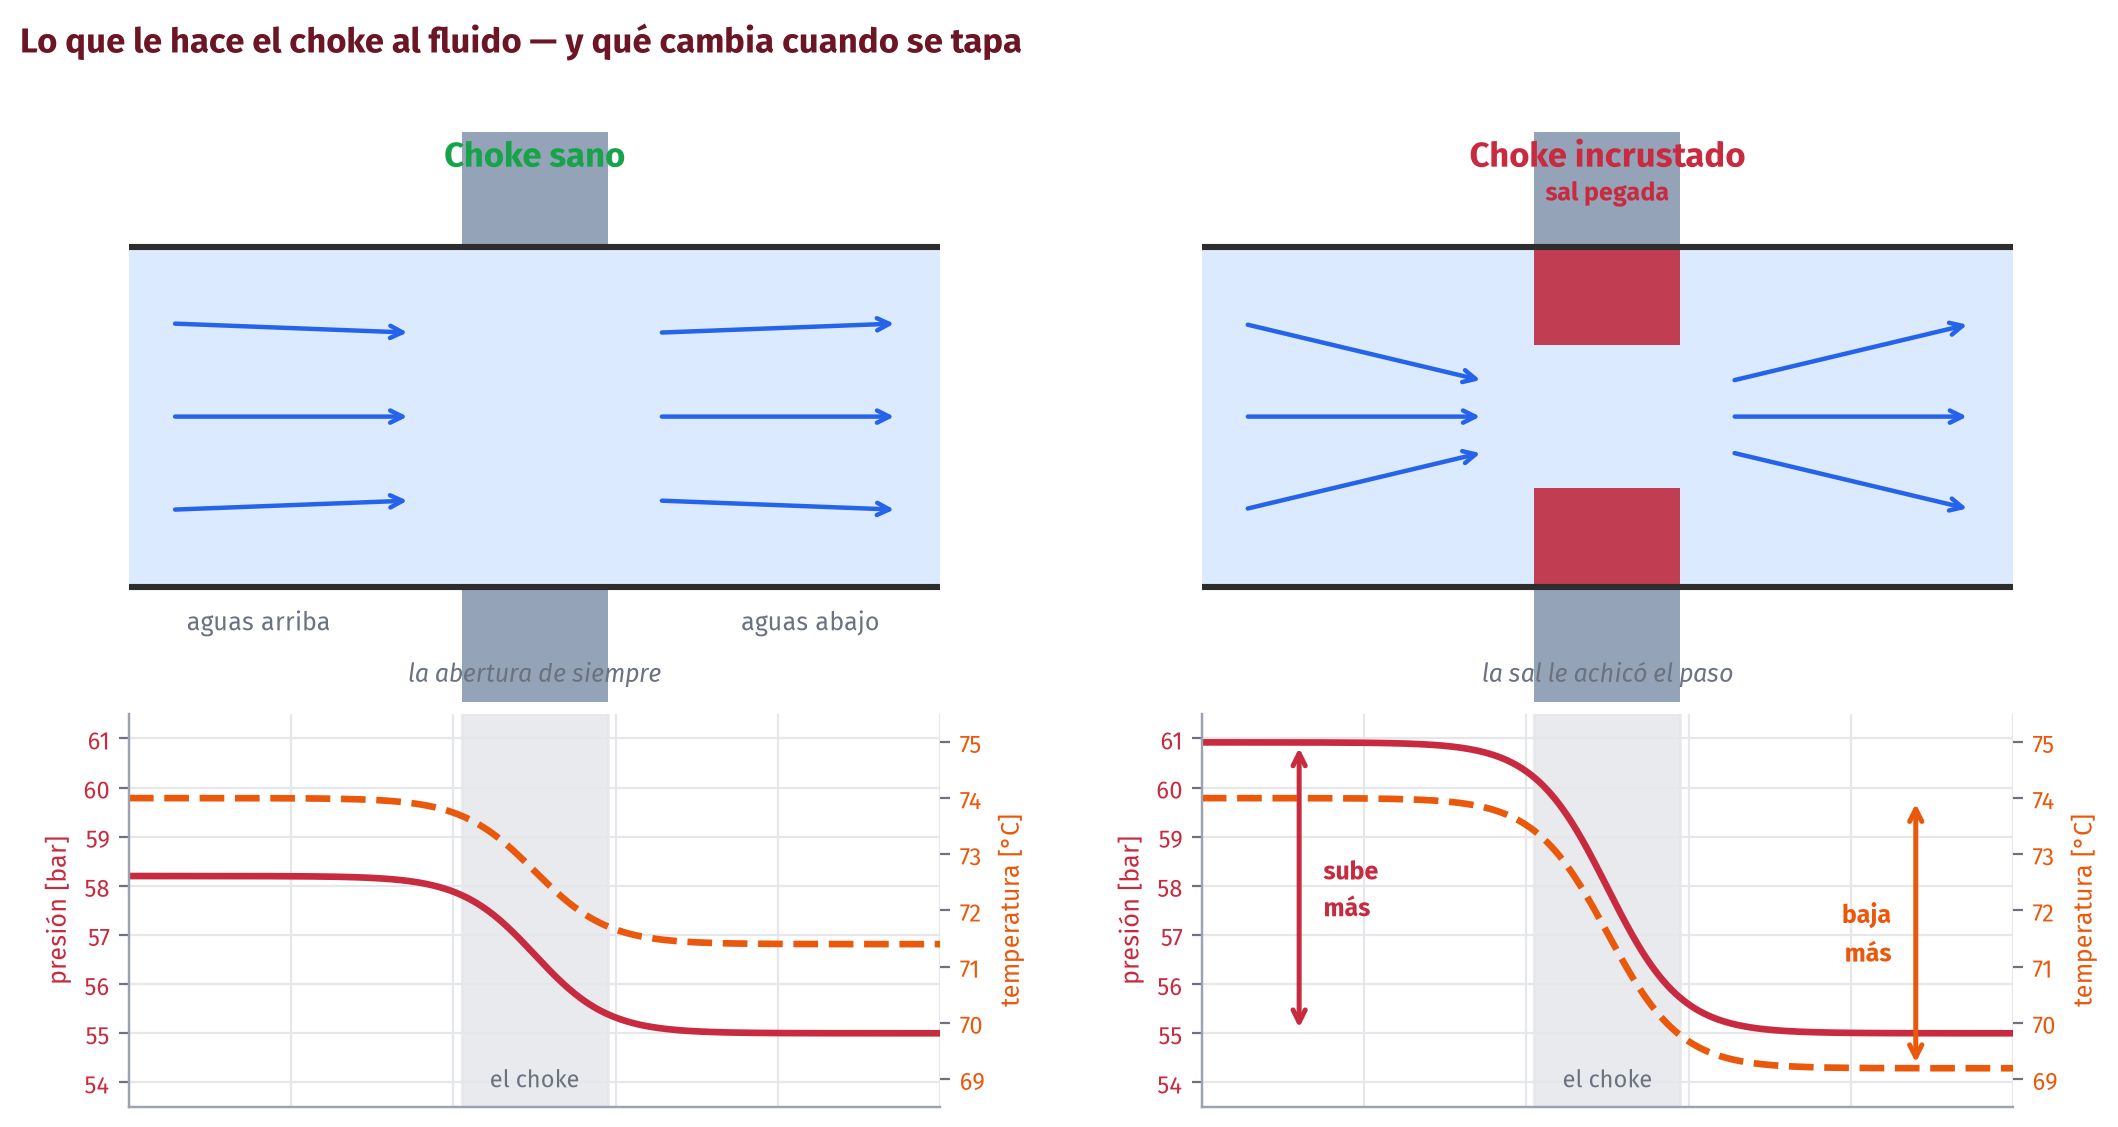
\includegraphics[height=0.70\textheight]{fig_choke.png}
  \end{center}
  \vspace{-4pt}
  {\footnotesize\color{arcaDark}
   Dos cosas pasan siempre que un fluido cruza un estrangulamiento:
   la presión \textbf{cae} de un lado al otro, y la temperatura
   \textbf{también}.}
\end{frame}

\begin{frame}[shrink=8]{Por Qué se Enfría: el Efecto Joule--Thomson}
  \vspace{-4pt}
  {\small\color{arcaDark}\bfseries
   Este es el fenómeno físico que hace posible toda la clase de hoy.
   No se puede dar por sabido.}
  \vspace{8pt}
  \begin{columns}[T]
    \begin{column}{0.51\textwidth}
      {\footnotesize\color{textMuted}
      Cuando un gas pasa de una zona de alta presión a una de baja presión
      \textbf{sin recibir calor de afuera}, se \textbf{expande}. Para
      expandirse tiene que empujar, y esa energía la saca de sí mismo.\\[6pt]
      Resultado: \textbf{se enfría}. Y cuanto mayor es la caída de presión,
      más se enfría.}
      \vspace{7pt}
      \begin{tcolorbox}[colback=arcaGray, colframe=codeBlue, boxrule=0pt, leftrule=3pt,
        arc=3pt, left=6pt, right=6pt, top=4pt, bottom=4pt]
        {\scriptsize\color{codeBlue}\bfseries\faSnowflake\hspace{4pt}LO VIERON MIL VECES}\\[4pt]
        {\scriptsize\color{textMuted}
         Una garrafa de gas que se está descargando se \textbf{escarcha}
         por fuera. Un aerosol se enfría en la mano. Es lo mismo: gas que se
         expande, gas que se enfría.}
      \end{tcolorbox}
    \end{column}
    \begin{column}{0.45\textwidth}
      {\small\color{arcaDark}\bfseries\faLink\hspace{5pt}La cadena completa}
      \vspace{5pt}
      {\footnotesize\color{textMuted}
      \begin{enumerate}\setlength{\itemsep}{4pt}
        \item El agujero del choke se achica
        \item Para pasar el mismo fluido por un agujero menor, hay que
              \textbf{empujar más} $\rightarrow$ la presión de antes
              \textbf{sube}
        \item La caída a través del choke es \textbf{mayor}
        \item Mayor caída $\rightarrow$ mayor expansión $\rightarrow$
              \textbf{más frío del otro lado}
      \end{enumerate}}
      \vspace{6pt}
      \begin{tcolorbox}[colback=arcaGray, colframe=arcaRed, boxrule=0pt, leftrule=3pt,
        arc=3pt, left=6pt, right=6pt, top=4pt, bottom=4pt]
        {\scriptsize\color{arcaRed}\bfseries\faKey\hspace{4pt}LA FIRMA A BUSCAR}\\[3pt]
        {\scriptsize\color{textMuted}
         Presión \textbf{arriba} subiendo \emph{y} temperatura
         \textbf{abajo} bajando, \textbf{al mismo tiempo}.}
      \end{tcolorbox}
    \end{column}
  \end{columns}
\end{frame}

\begin{frame}[shrink=8]{Qué es la Incrustación, y Por Qué se Ve en la Presión}
  \vspace{-4pt}
  \begin{columns}[T]
    \begin{column}{0.50\textwidth}
      {\small\color{arcaDark}\bfseries\faQuestion\hspace{5pt}Qué pasa físicamente}
      \vspace{4pt}
      {\footnotesize\color{textMuted}
      El agua de formación trae sales disueltas (carbonatos, sulfatos).
      Al pasar por el choke la presión cae de golpe, la sal precipita
      y se \textbf{pega a las paredes}.\\[5pt]
      El agujero por donde pasa el fluido se va \textbf{achicando}.
      Nadie lo abrió ni lo cerró: se cerró solo.}
      \vspace{7pt}
      \begin{tcolorbox}[colback=arcaGray, colframe=arcaRed, boxrule=0pt, leftrule=3pt,
        arc=3pt, left=6pt, right=6pt, top=5pt, bottom=5pt]
        {\scriptsize\color{arcaRed}\bfseries\faLightbulb[regular]\hspace{4pt}LA CLAVE DE HOY}\\[4pt]
        {\scriptsize\color{textMuted}
         La incrustación \textbf{no es un evento}: es un proceso que tarda
         horas. Por eso se puede ver venir --- si uno sabe dónde mirar.}
      \end{tcolorbox}
    \end{column}
    \begin{column}{0.46\textwidth}
      {\small\color{arcaDark}\bfseries\faEye\hspace{5pt}Qué deja como huella}
      \vspace{4pt}
      {\footnotesize\color{textMuted}
      \begin{itemize}\setlength{\itemsep}{6pt}
        \item[{\color{arcaRed}\scriptsize\faArrowUp}]
          \textbf{Aguas arriba} del choke la presión \textbf{sube}:
          el fluido empuja contra una salida más chica.
        \item[{\color{codeBlue}\scriptsize\faArrowDown}]
          \textbf{Aguas abajo} la temperatura \textbf{baja}: al estrangular más,
          el gas se expande más y se enfría más
          (el mismo efecto que enfría una garrafa cuando se descarga).
      \end{itemize}}
      \vspace{6pt}
      {\scriptsize\color{arcaDark}\itshape
        Guarden estas dos flechas. Dentro de tres láminas las vamos a ver
        pasar, en un pozo de verdad.}
    \end{column}
  \end{columns}
\end{frame}

\begin{frame}[shrink=8]{Qué es, Exactamente, una Serie de Tiempo}
  \vspace{-4pt}
  {\small\color{arcaDark}\bfseries
   Una tabla donde cada fila es un instante, y las filas están en orden.
   Eso es todo. Lo difícil es lo que implica.}
  \vspace{5pt}
  \begin{center}
    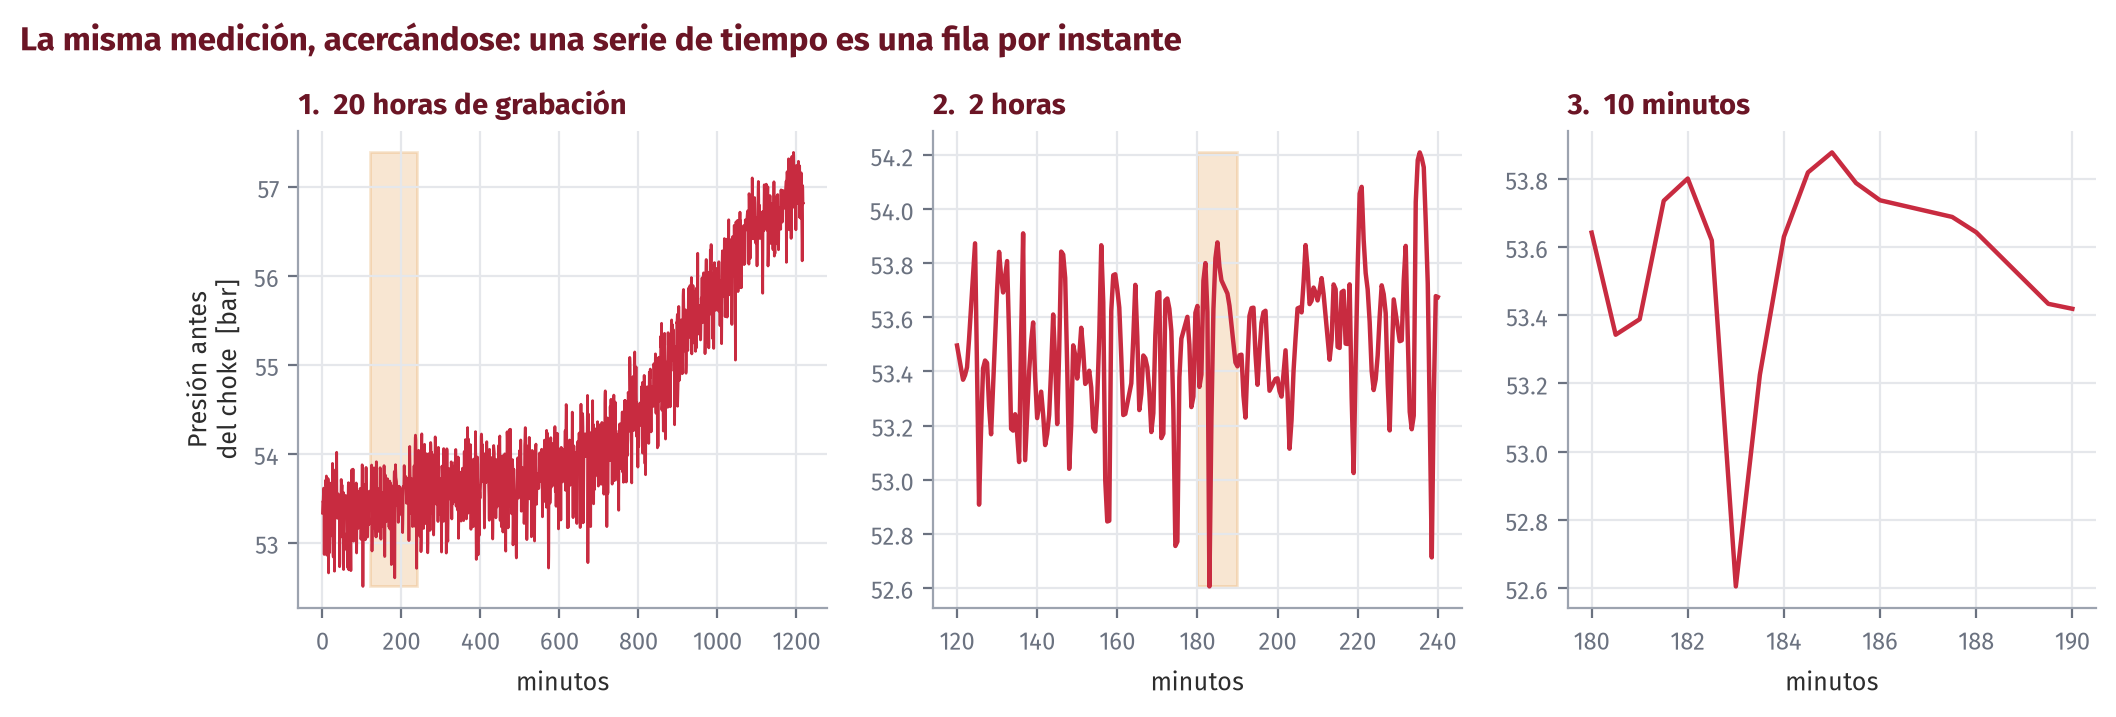
\includegraphics[height=0.50\textheight]{fig_que_es_serie.png}
  \end{center}
  \vspace{-2pt}
  \begin{columns}[T]
    \begin{column}{0.49\textwidth}
      {\footnotesize\color{textMuted}
      \begin{itemize}\setlength{\itemsep}{2pt}
        \item[{\color{arcaRed}\scriptsize\faArrowRight}]
          El sensor mide \textbf{una vez por segundo}: 86\,400 filas por día,
          por sensor, por pozo.
        \item[{\color{arcaRed}\scriptsize\faArrowRight}]
          Nosotros nos quedamos con \textbf{una cada 30 segundos}: la
          incrustación tarda horas, el resto es peso.
      \end{itemize}}
    \end{column}
    \begin{column}{0.49\textwidth}
      \begin{tcolorbox}[colback=arcaGray, colframe=arcaDark, boxrule=0pt, leftrule=3pt,
        arc=3pt, left=6pt, right=6pt, top=4pt, bottom=4pt]
        {\scriptsize\color{arcaDark}\bfseries\faExclamationTriangle\hspace{4pt}LA REGLA DEL MÓDULO}\\[3pt]
        {\scriptsize\color{textMuted}
         Ningún cálculo puede usar información que no existía en el momento
         que se está describiendo. Si la usa, el modelo adivina el futuro
         en el cuaderno y falla en el pozo.}
      \end{tcolorbox}
    \end{column}
  \end{columns}
\end{frame}

\begin{frame}[fragile, shrink=20]{El Archivo: Qué Hay Adentro}
  \vspace{-4pt}
  \begin{columns}[T]
    \begin{column}{0.56\textwidth}
      \begin{pyblock}
import pandas as pd

URL = ("https://raw.githubusercontent.com/"
       "cmosquerat/slb-diplomado/main/"
       "datos/pozos_3w_incrustacion.csv")

# leemos el archivo (se baja solo)
d = pd.read_csv(URL)

# ¿cuantas filas y cuantas columnas?
print(d.shape)

# ¿cuantas grabaciones hay, y de que pozos?
print(d.pozo.value_counts())
      \end{pyblock}
    \end{column}
    \begin{column}{0.42\textwidth}
      \vspace{2pt}
      \begin{outputblock}
(37822, 9)

WELL-00023    16901
WELL-00024    11772
WELL-00022     3780
WELL-00021     2926
WELL-00001     2443
      \end{outputblock}
      \vspace{4pt}
      {\footnotesize\color{textMuted}
      \begin{itemize}\setlength{\itemsep}{3pt}
        \item[{\color{arcaRed}\scriptsize\faDatabase}]
          \textbf{315 horas} de pozo grabadas
        \item[{\color{arcaRed}\scriptsize\faIndustry}]
          \textbf{5 pozos}, \textbf{12 grabaciones}
        \item[{\color{codeGreen}\scriptsize\faCheck}]
          Datos \textbf{reales}: ni simulados ni dibujados
      \end{itemize}}
    \end{column}
  \end{columns}
\end{frame}

\begin{frame}[shrink=10]{Las Variables, Una a Una}
  \vspace{-4pt}
  {\footnotesize
  \renewcommand{\arraystretch}{1.2}
  \begin{tabular}{@{}p{3.1cm}p{2.5cm}p{9.1cm}@{}}
    \toprule
    {\color{arcaDark}\bfseries columna} &
    {\color{arcaDark}\bfseries tag de campo} &
    {\color{arcaDark}\bfseries qué es} \\
    \midrule
    \texttt{p\_antes\_choke} & P-MON-CKP &
      Presión justo \emph{antes} de la válvula. Sube si la válvula se tapa \\
    \texttt{t\_despues\_choke} & T-JUS-CKP &
      Temperatura justo \emph{después}. Baja si la válvula se tapa \\
    \texttt{p\_arbol} & P-TPT &
      Presión en el árbol submarino, en la boca del pozo \\
    \texttt{p\_anular} & P-ANULAR &
      Presión en el espacio entre tuberías. Vigila la integridad \\
    \texttt{p\_gaslift} & P-JUS-CKGL &
      Presión del gas que se inyecta para aligerar la columna \\
    \midrule
    \rowcolor{arcaGray}
    \texttt{etiqueta} & \emph{class} &
      {\color{arcaRed}\bfseries Lo que hay que predecir.} La puso una persona,
      no un sensor \\
    \bottomrule
  \end{tabular}}
  \vspace{8pt}

  {\scriptsize\color{textMuted}\itshape
   Cinco columnas, y las cinco se explican en una línea. Ese fue un criterio
   para elegir este dataset: si una variable necesita un párrafo, la clase
   se va a hablar de la variable y no del problema.}
\end{frame}

\begin{frame}[shrink=8]{Qué es una Etiqueta, y Quién la Puso}
  \vspace{-4pt}
  {\small\color{arcaDark}\bfseries
   Esta es la lámina más importante del día, y no tiene ni una fórmula.}
  \vspace{7pt}
  \begin{columns}[T]
    \begin{column}{0.53\textwidth}
      {\footnotesize\color{textMuted}
      La columna \texttt{etiqueta} toma tres valores:
      \vspace{5pt}
      \begin{itemize}\setlength{\itemsep}{5pt}
        \item[{\color{codeGreen}\scriptsize\faCheck}]
          \textbf{\texttt{normal}} --- el pozo trabajando bien
        \item[{\color{codeOrange}\scriptsize\faExclamationTriangle}]
          \textbf{\texttt{transitorio}} --- la incrustación \emph{avanzando}.
          Todavía se puede hacer algo
        \item[{\color{arcaRed}\scriptsize\faTimes}]
          \textbf{\texttt{falla}} --- ya está. Se acabó la ventana
      \end{itemize}}
      \vspace{7pt}
      {\footnotesize\color{arcaDark}
       Nuestro objetivo es \textbf{cazar el naranja}: avisar durante el
       transitorio, que es cuando el aviso todavía sirve.}
    \end{column}
    \begin{column}{0.44\textwidth}
      \begin{tcolorbox}[colback=arcaGray, colframe=arcaRed, boxrule=0pt, leftrule=3pt,
        arc=3pt, left=6pt, right=6pt, top=5pt, bottom=5pt]
        {\scriptsize\color{arcaRed}\bfseries\faUserEdit\hspace{4pt}LA ETIQUETA ES UN JUICIO}\\[4pt]
        {\scriptsize\color{textMuted}
         Estas etiquetas las escribieron \textbf{especialistas de Petrobras}
         mirando las grabaciones, segundo a segundo.\\[4pt]
         No son la verdad: son \textbf{la opinión de una persona experta}.
         Alguien decidió en qué segundo exacto «empieza» algo que en realidad
         empezó de a poco.}
      \end{tcolorbox}
      \vspace{5pt}
      {\scriptsize\color{arcaDark}\itshape
        Anótenlo. Al final de la clase esto nos va a pasar factura ---
        y va a ser la mejor noticia del día.}
    \end{column}
  \end{columns}
\end{frame}

\begin{frame}[shrink=6]{La Señal, de Verdad}
  \vspace{-8pt}
  \begin{center}
    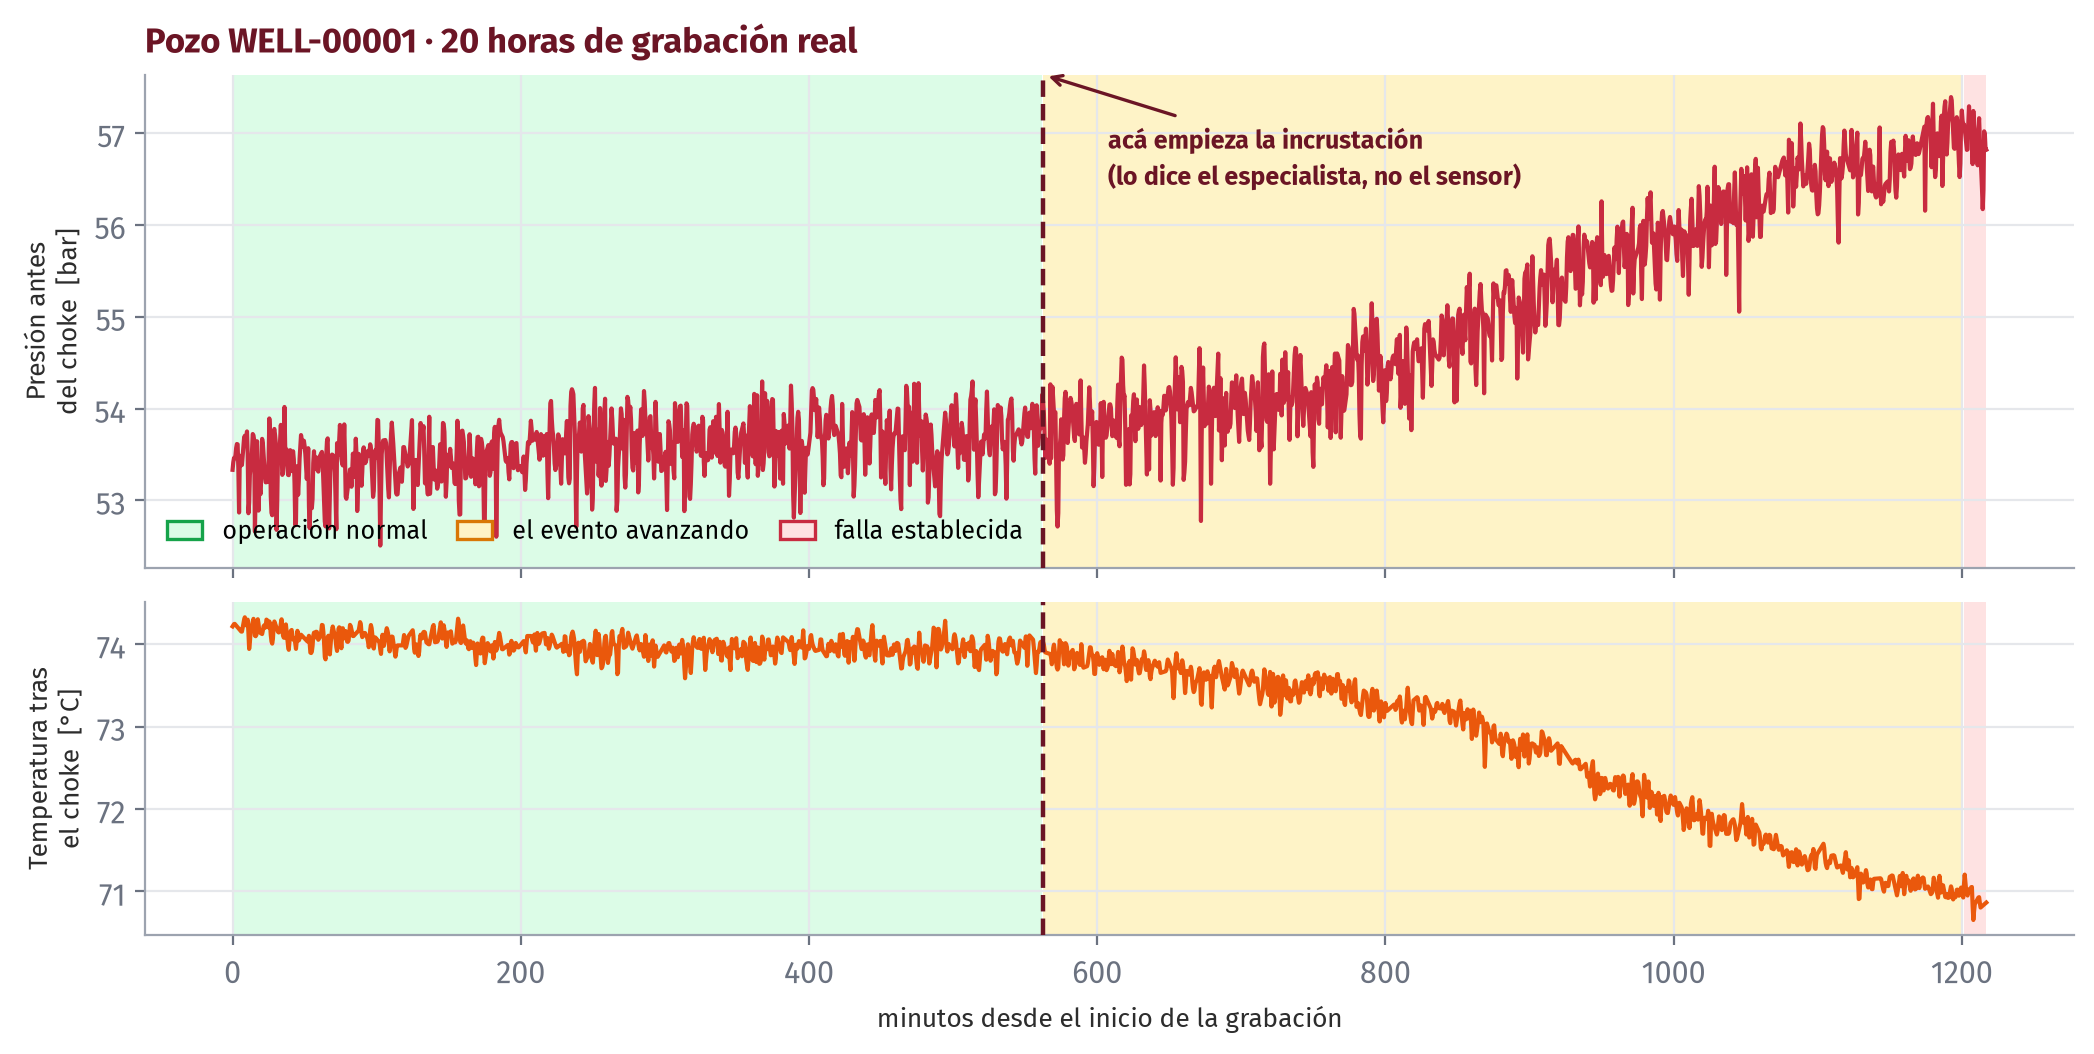
\includegraphics[height=0.72\textheight]{fig_senal_cruda.png}
  \end{center}
  \vspace{-6pt}
  {\footnotesize\color{arcaDark}
   Ahí están las dos flechas que anotamos: la presión de arriba \textbf{sube},
   la temperatura de abajo \textbf{baja}. La física se ve a simple vista.}
\end{frame}

\begin{frame}[shrink=8]{Lo Primero que Hace un Ingeniero: Mirar Qué Hay}
  \vspace{-4pt}
  \begin{columns}[T]
    \begin{column}{0.62\textwidth}
      \vspace{-2pt}
      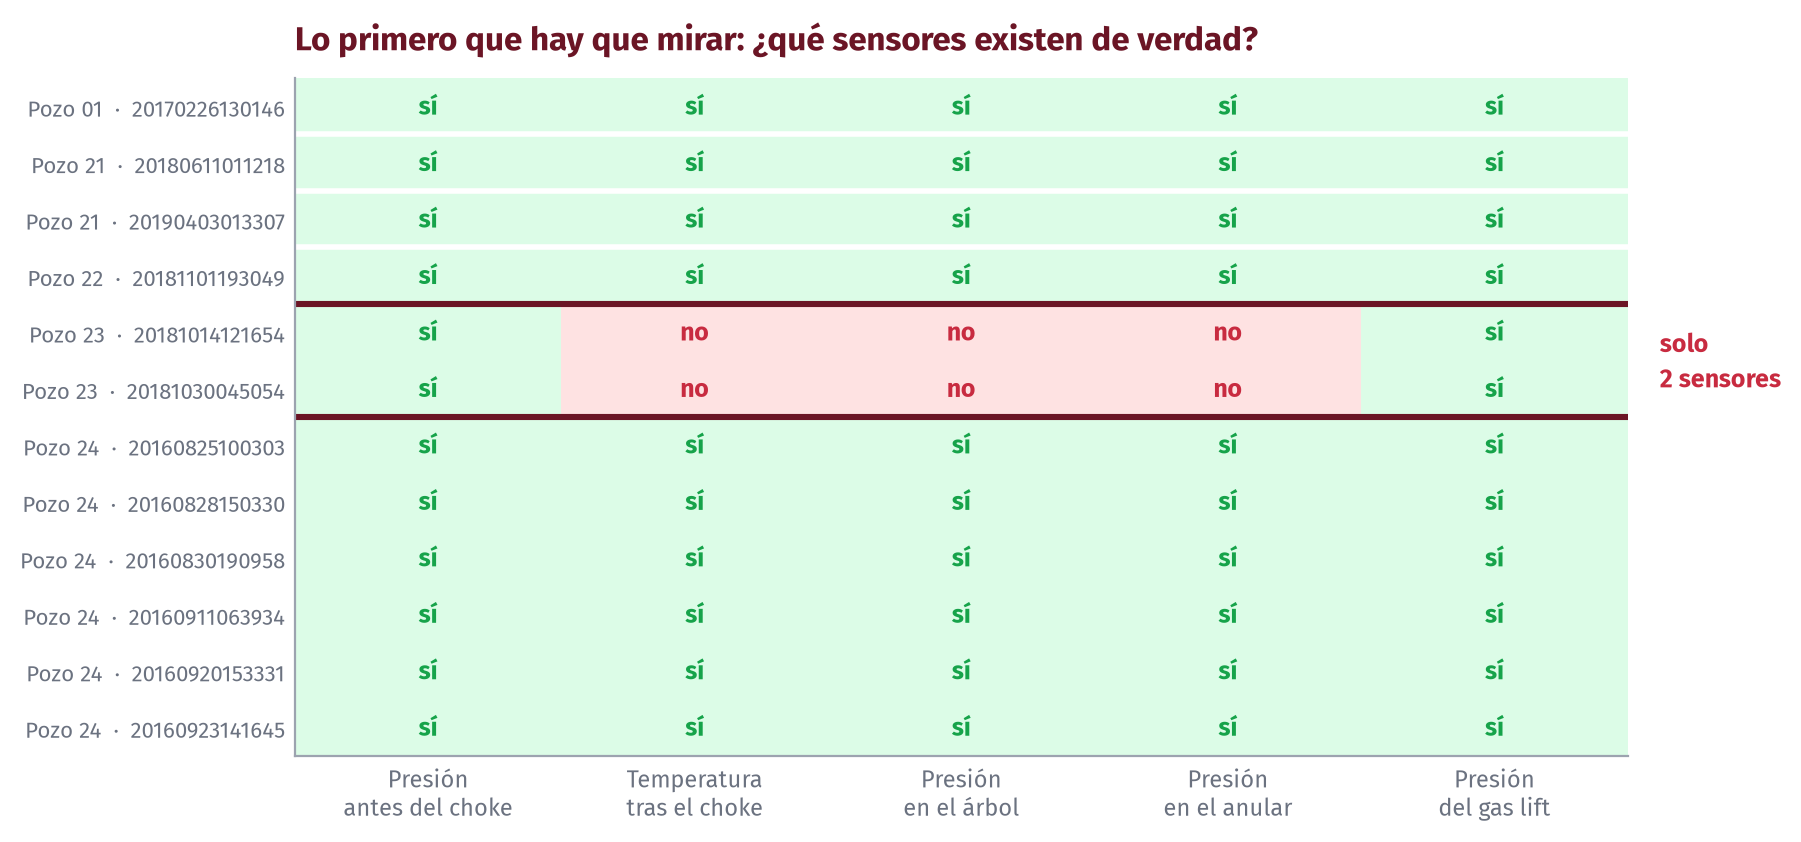
\includegraphics[width=\textwidth]{fig_sensores.png}
    \end{column}
    \begin{column}{0.35\textwidth}
      {\footnotesize\color{textMuted}
      Antes de modelar nada: \textbf{¿qué sensores existen realmente?}
      \vspace{6pt}
      \begin{itemize}\setlength{\itemsep}{4pt}
        \item[{\color{arcaRed}\scriptsize\faExclamationTriangle}]
          El \textbf{pozo 23} tiene solo \textbf{dos} sensores vivos.
          Los otros tres están en el archivo, pero vacíos.
        \item[{\color{arcaRed}\scriptsize\faArrowRight}]
          Esto no es un defecto del dataset. Es \textbf{cómo son los datos
          de campo}: sensores rotos, no instalados, o que dejaron de reportar.
      \end{itemize}}
      \vspace{6pt}
      {\scriptsize\color{arcaDark}\itshape
        Decisión que tomamos acá, en voz alta: el pozo 23 queda \textbf{fuera}
        de la clase, y va a ser el reto de la práctica.}
    \end{column}
  \end{columns}
\end{frame}

% ═════════════════════════════════════════════════════════════════════════════
\sectionframe{La Alarma que Ya Existe}{Antes de proponer nada nuevo, hay que medir lo que ya está instalado \\[6pt] \normalsize 42 -- 55 min}
% ═════════════════════════════════════════════════════════════════════════════

\begin{frame}[shrink=8]{Cómo Funciona una Alarma de Umbral}
  \vspace{-4pt}
  {\small\color{arcaDark}\bfseries
   Es la lógica más vieja de una sala de control, y funciona así:}
  \vspace{7pt}
  \begin{columns}[T]
    \begin{column}{0.47\textwidth}
      {\footnotesize\color{textMuted}
      \begin{enumerate}\setlength{\itemsep}{5pt}
        \item Se mira una hora de operación normal del pozo y se anota
              cuánto vale la presión \textbf{en promedio}.
        \item Se anota también \textbf{cuánto se mueve} alrededor de ese
              promedio: eso es la \textbf{desviación estándar}.
        \item Se dibuja una banda: promedio $\pm$ tres desviaciones.
        \item Si la señal se sale de la banda, \textbf{suena}.
      \end{enumerate}}
    \end{column}
    \begin{column}{0.49\textwidth}
      \begin{tcolorbox}[colback=arcaGray, colframe=codeBlue, boxrule=0pt, leftrule=3pt,
        arc=3pt, left=6pt, right=6pt, top=5pt, bottom=5pt]
        {\scriptsize\color{codeBlue}\bfseries\faRuler\hspace{4pt}QUÉ ES LA DESVIACIÓN ESTÁNDAR}\\[4pt]
        {\scriptsize\color{textMuted}
         Es una regla para medir «qué tan raro es un número» \textbf{en las
         unidades de ese pozo}.\\[4pt]
         Si la presión de un pozo normalmente se mueve $\pm$0{,}3 bar,
         entonces subir 1 bar es \textbf{muchísimo}. Si otro pozo se mueve
         $\pm$5 bar, subir 1 bar no es nada.\\[4pt]
         Contar «cuántas desviaciones» es preguntar \textbf{cuán raro es esto
         para este pozo}, no cuántos bar son.}
      \end{tcolorbox}
      \vspace{4pt}
      {\scriptsize\color{arcaDark}\itshape
        Tres desviaciones es la costumbre de la industria. Ni magia,
        ni teorema: costumbre.}
    \end{column}
  \end{columns}
\end{frame}

\begin{frame}[fragile, shrink=22]{La Alarma, en Código}
  \vspace{-4pt}
  \begin{columns}[T]
    \begin{column}{0.60\textwidth}
      \begin{pyblock}
pozo = "WELL-00001_20170226130146"
g = d[d.instancia == pozo]    # tomamos UN pozo

# la primera hora es su "normal"
# (120 filas = 120 x 30 s = 1 hora)
primera_hora = g.p_antes_choke.iloc[:120]

centro = primera_hora.median()   # valor tipico
ancho  = primera_hora.std()      # cuanto se mueve

# cuantas desviaciones de distancia hay
# en cada instante
z = (g.p_antes_choke - centro) / ancho

# la alarma suena si se pasa de 3
suena = z.abs() > 3
      \end{pyblock}
    \end{column}
    \begin{column}{0.38\textwidth}
      \vspace{2pt}
      {\footnotesize\color{textMuted}
      Fíjense en lo que hicimos con \texttt{z}:
      \vspace{5pt}
      \begin{itemize}\setlength{\itemsep}{4pt}
        \item[{\color{arcaRed}\scriptsize\faArrowRight}]
          restamos el centro $\rightarrow$ ahora 0 significa
          \textbf{«normal para este pozo»}
        \item[{\color{arcaRed}\scriptsize\faArrowRight}]
          dividimos por el ancho $\rightarrow$ ahora 1 significa
          \textbf{«un temblor típico de este pozo»}
      \end{itemize}}
      \vspace{6pt}
      \begin{tcolorbox}[colback=arcaGray, colframe=arcaRed, boxrule=0pt, leftrule=3pt,
        arc=3pt, left=6pt, right=6pt, top=4pt, bottom=4pt]
        {\scriptsize\color{textMuted}
         Esas dos líneas van a ser, dentro de media hora, \textbf{el
         hallazgo de toda la clase}. Todavía no lo saben.}
      \end{tcolorbox}
    \end{column}
  \end{columns}
\end{frame}

\begin{frame}[shrink=6]{La Alarma, Puesta a Prueba en un Pozo}
  \vspace{-8pt}
  \begin{center}
    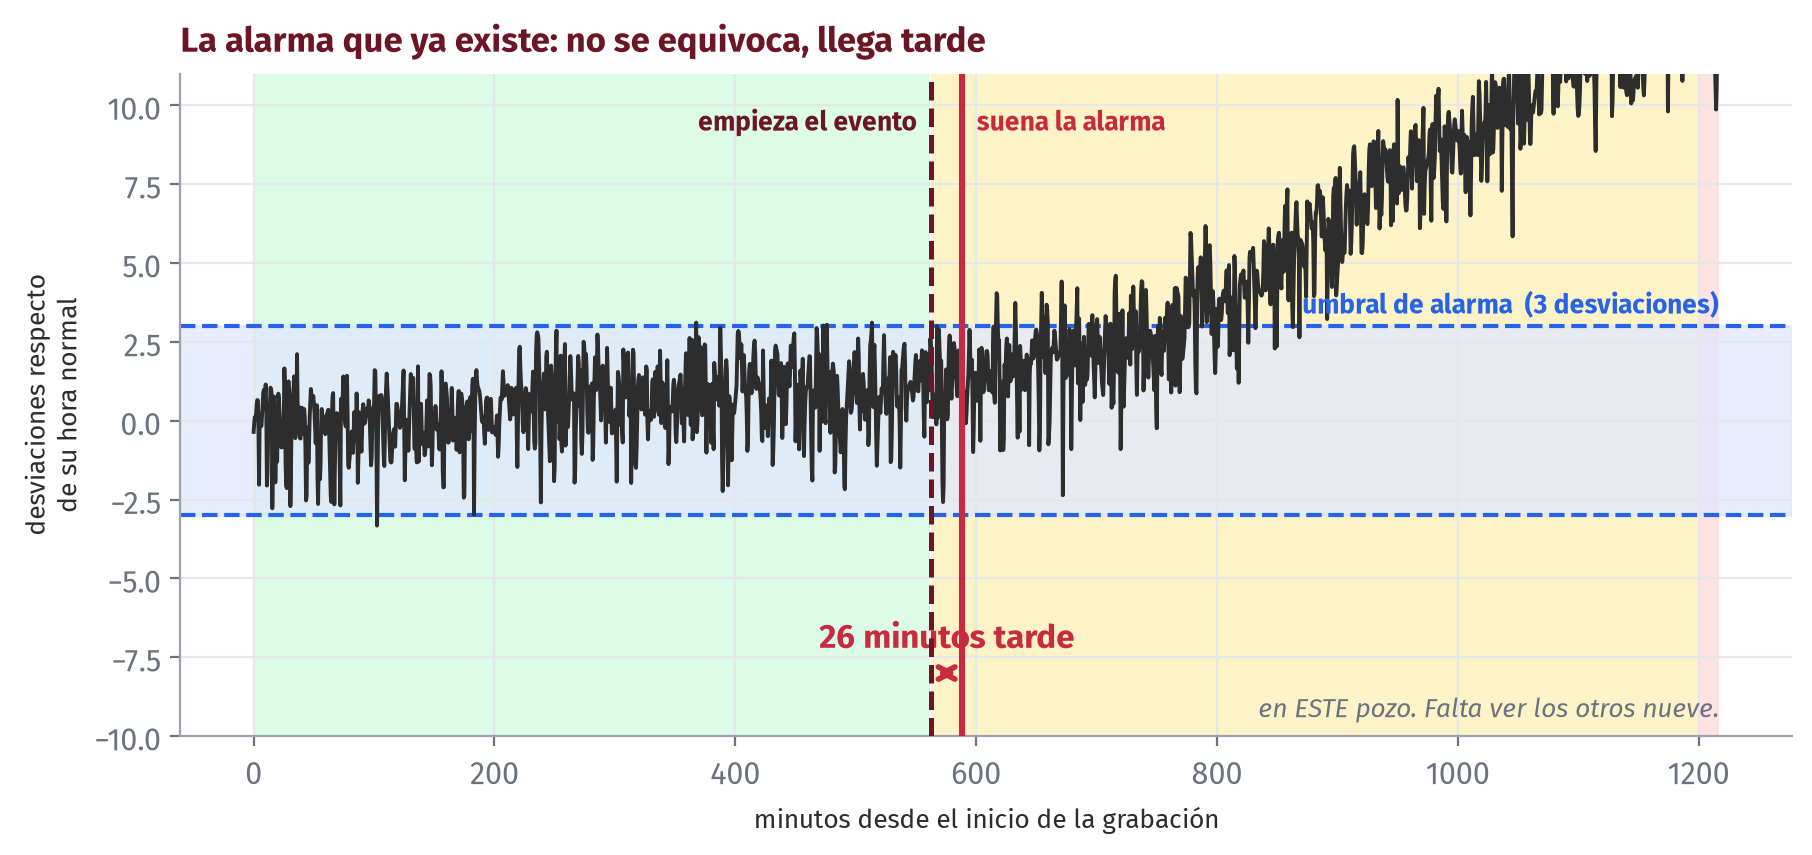
\includegraphics[height=0.66\textheight]{fig_alarma.png}
  \end{center}
  \vspace{-4pt}
  {\footnotesize\color{textMuted}
   La alarma \textbf{no se equivocó}: la presión efectivamente se salió de la
   banda. El problema es \emph{cuándo}. Y en este pozo, dicho sea de paso,
   no lo hace mal.}
\end{frame}

\begin{frame}[shrink=8]{Cómo se Mide «Bien» o «Mal»: Tres Números}
  \vspace{-4pt}
  {\small\color{arcaDark}\bfseries
   Si no definimos esto ahora, después cada uno defiende el número que le
   conviene.}
  \vspace{7pt}
  {\footnotesize
  \renewcommand{\arraystretch}{1.35}
  \begin{tabular}{@{}p{3.7cm}p{10.7cm}@{}}
    \toprule
    {\color{arcaDark}\bfseries Casos detectados} &
      De los 10 eventos grabados, \textbf{¿en cuántos avisó alguna vez?}
      Si no avisa nunca, el resto no importa \\
    {\color{arcaDark}\bfseries Retraso} &
      \textbf{¿Cuántos minutos pasaron} desde que el evento empezó hasta el
      primer aviso? Menos es mejor \\
    {\color{arcaDark}\bfseries Falsas alarmas} &
      \textbf{¿Qué porcentaje del tiempo normal} estuvo gritando sin motivo?
      Una alarma que grita siempre se apaga, y entonces no sirve para nada \\
    \bottomrule
  \end{tabular}}
  \vspace{9pt}

  \begin{tcolorbox}[colback=arcaGray, colframe=arcaRed, boxrule=0pt, leftrule=3pt,
    arc=3pt, left=8pt, right=8pt, top=5pt, bottom=5pt]
    {\scriptsize\color{arcaRed}\bfseries\faBalanceScale\hspace{4pt}LA REGLA DE COMPARACIÓN JUSTA}\\[4pt]
    {\scriptsize\color{textMuted}
     Los tres números se mueven juntos: cualquiera detecta más si acepta
     gritar más. Por eso, \textbf{todo lo que comparemos hoy va a estar
     obligado a la misma tasa de falsas alarmas que la alarma actual}.
     Comparar a distinta tasa de falsas alarmas es hacer trampa.}
  \end{tcolorbox}
\end{frame}

\begin{frame}[shrink=8]{El Récord a Batir}
  \vspace{-4pt}
  {\small\color{arcaDark}\bfseries
   Corrimos la alarma sobre las 10 grabaciones. Este es el número que hay
   que superar:}
  \vspace{10pt}
  \begin{columns}[T]
    \begin{column}{0.31\textwidth}
      \begin{tcolorbox}[colback=arcaGray, colframe=arcaDark, boxrule=0pt, leftrule=3pt,
        arc=3pt, left=6pt, right=6pt, top=6pt, bottom=6pt]
        \centering
        {\scriptsize\color{textMuted}CASOS DETECTADOS}\\[4pt]
        {\LARGE\color{arcaDark}\bfseries 8 de 10}\\[4pt]
        {\scriptsize\color{textMuted}dos eventos completos\\se le pasaron enteros}
      \end{tcolorbox}
    \end{column}
    \begin{column}{0.31\textwidth}
      \begin{tcolorbox}[colback=arcaGray, colframe=arcaRed, boxrule=0pt, leftrule=3pt,
        arc=3pt, left=6pt, right=6pt, top=6pt, bottom=6pt]
        \centering
        {\scriptsize\color{textMuted}RETRASO (MEDIANA)}\\[4pt]
        {\LARGE\color{arcaRed}\bfseries 101 min}\\[4pt]
        {\scriptsize\color{textMuted}casi dos horas\\después de empezar}
      \end{tcolorbox}
    \end{column}
    \begin{column}{0.31\textwidth}
      \begin{tcolorbox}[colback=arcaGray, colframe=codeBlue, boxrule=0pt, leftrule=3pt,
        arc=3pt, left=6pt, right=6pt, top=6pt, bottom=6pt]
        \centering
        {\scriptsize\color{textMuted}FALSAS ALARMAS}\\[4pt]
        {\LARGE\color{codeBlue}\bfseries 13{,}5 \%}\\[4pt]
        {\scriptsize\color{textMuted}este es el presupuesto\\que nadie puede pasar}
      \end{tcolorbox}
    \end{column}
  \end{columns}
  \vspace{10pt}
  {\footnotesize\color{arcaDark}\itshape
   Ahora sí sabemos contra qué jugamos. Y noten que la alarma \textbf{no es
   mala}: detecta 8 de 10. El problema es que avisa cuando ya casi no queda
   nada por hacer.}
\end{frame}

% ═════════════════════════════════════════════════════════════════════════════
\sectionframe{De la Señal a una Tabla}{Los modelos no comen señales: comen tablas. Hay que traducir. \\[6pt] \normalsize 55 -- 82 min}
% ═════════════════════════════════════════════════════════════════════════════

\begin{frame}[shrink=8]{El Problema de Traducción}
  \vspace{-4pt}
  \begin{columns}[T]
    \begin{column}{0.47\textwidth}
      {\small\color{arcaDark}\bfseries\faTimes\hspace{5pt}Lo que tenemos}
      \vspace{4pt}
      {\footnotesize\color{textMuted}
      Una \textbf{señal}: 37\,822 mediciones en fila india, donde el
      significado de cada número depende de los que vinieron antes.\\[5pt]
      Un valor de 54 bar no dice nada. \textbf{54 bar después de venir de 53
      durante ocho horas} lo dice todo.}
    \end{column}
    \begin{column}{0.47\textwidth}
      {\small\color{arcaDark}\bfseries\faCheck\hspace{5pt}Lo que come el modelo}
      \vspace{4pt}
      {\footnotesize\color{textMuted}
      Una \textbf{tabla}: filas independientes, donde cada fila se explica
      sola y el orden no importa.\\[5pt]
      Es la misma tabla del Módulo 3: una fila por caso, una columna por
      característica, una etiqueta al final.}
    \end{column}
  \end{columns}
  \vspace{10pt}
  \begin{tcolorbox}[colback=arcaGray, colframe=arcaRed, boxrule=0pt, leftrule=3pt,
    arc=3pt, left=8pt, right=8pt, top=6pt, bottom=6pt]
    {\small\color{arcaRed}\bfseries\faTools\hspace{5pt}EL TRABAJO DE ESTE BLOQUE}\\[5pt]
    {\footnotesize\color{textMuted}
     Meterle a cada fila, en sus columnas, \textbf{el contexto que la señal
     tenía en el tiempo}. Si lo hacemos bien, el modelo no necesita saber que
     esto era una serie de tiempo.}
  \end{tcolorbox}
\end{frame}

\begin{frame}[shrink=4]{Descomponer: Toda Señal es una Suma de Tres Cosas}
  \vspace{-10pt}
  \begin{center}
    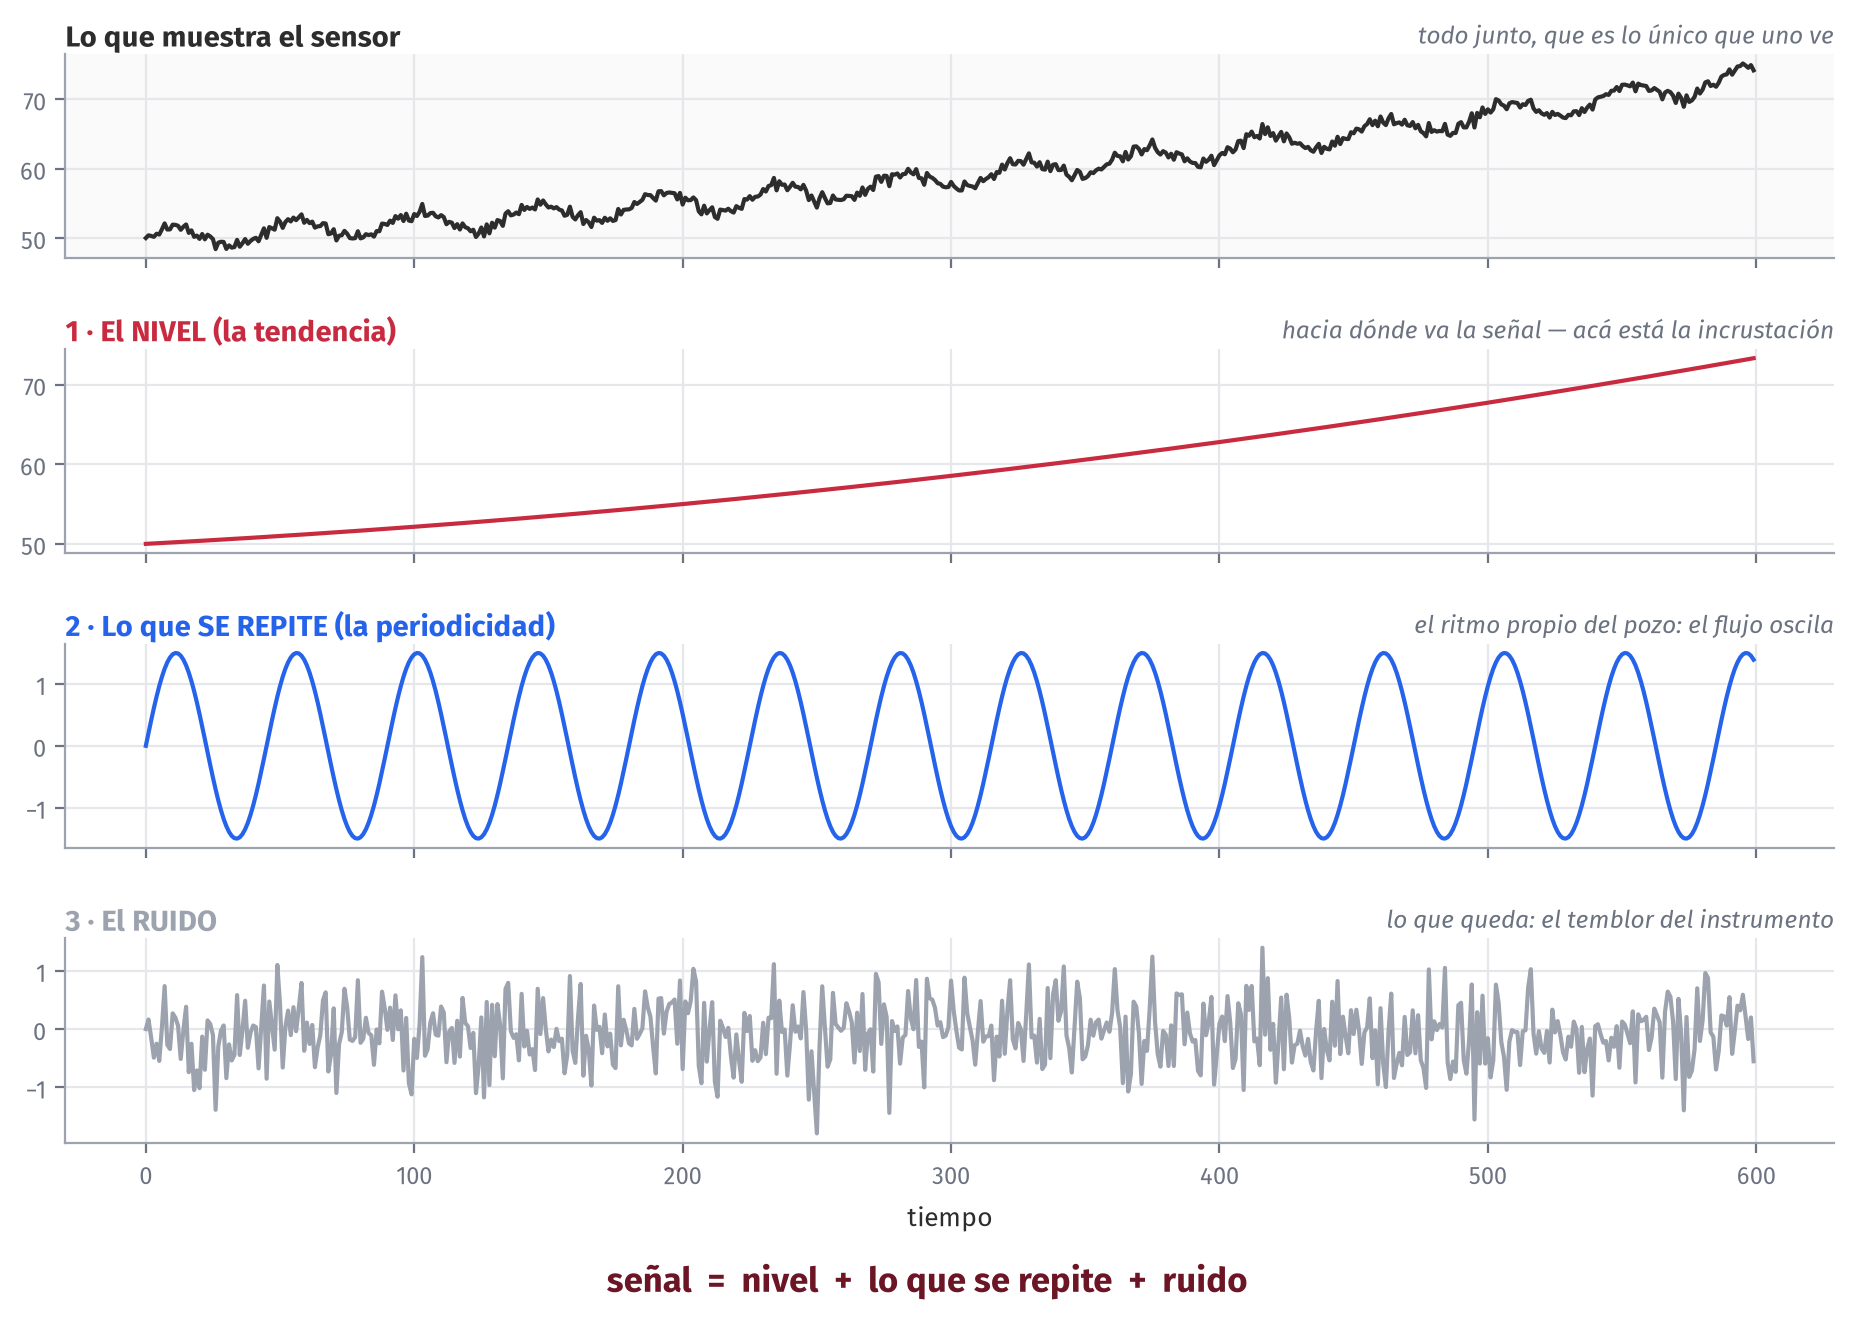
\includegraphics[height=0.86\textheight]{fig_tres_componentes.png}
  \end{center}
\end{frame}

\begin{frame}[shrink=8]{Las Tres Componentes, Una a Una}
  \vspace{-4pt}
  {\small\color{arcaDark}\bfseries
   Ninguna es «la buena»: son tres preguntas distintas sobre el pozo.}
  \vspace{6pt}
  {\footnotesize
  \renewcommand{\arraystretch}{1.4}
  \begin{tabular}{@{}p{2.6cm}p{4.3cm}p{7.4cm}@{}}
    \toprule
    {\color{arcaDark}\bfseries componente} &
    {\color{arcaDark}\bfseries cómo se calcula} &
    {\color{arcaDark}\bfseries qué pregunta contesta} \\
    \midrule
    {\color{arcaRed}\bfseries El nivel} &
      El \textbf{promedio} de la última media hora &
      ¿Dónde está parada la señal? Acá vive la incrustación \\
    {\color{codeBlue}\bfseries El ruido} &
      La \textbf{desviación estándar} de esa misma media hora &
      ¿Cuánto tiembla? Un pozo tapándose se vuelve más inestable \\
    {\color{codeGreen}\bfseries La pendiente} &
      El valor de ahora \textbf{menos} el de media hora atrás &
      ¿Hacia dónde va, y qué tan rápido? \\
    \bottomrule
  \end{tabular}}
  \vspace{9pt}

  \begin{tcolorbox}[colback=arcaGray, colframe=arcaDark, boxrule=0pt, leftrule=3pt,
    arc=3pt, left=8pt, right=8pt, top=5pt, bottom=5pt]
    {\scriptsize\color{arcaDark}\bfseries\faQuestion\hspace{4pt}QUÉ ES UN PROMEDIO MÓVIL}\\[4pt]
    {\scriptsize\color{textMuted}
     El promedio de siempre, pero sobre una ventana que \textbf{se va
     corriendo}: para cada instante se miran los últimos 30 minutos y se
     promedia. Sirve para \textbf{sacarle el temblor a la señal}.}
  \end{tcolorbox}
\end{frame}

\begin{frame}[shrink=6]{La Ventana Deslizante: el Truco Completo}
  \vspace{-8pt}
  \begin{center}
    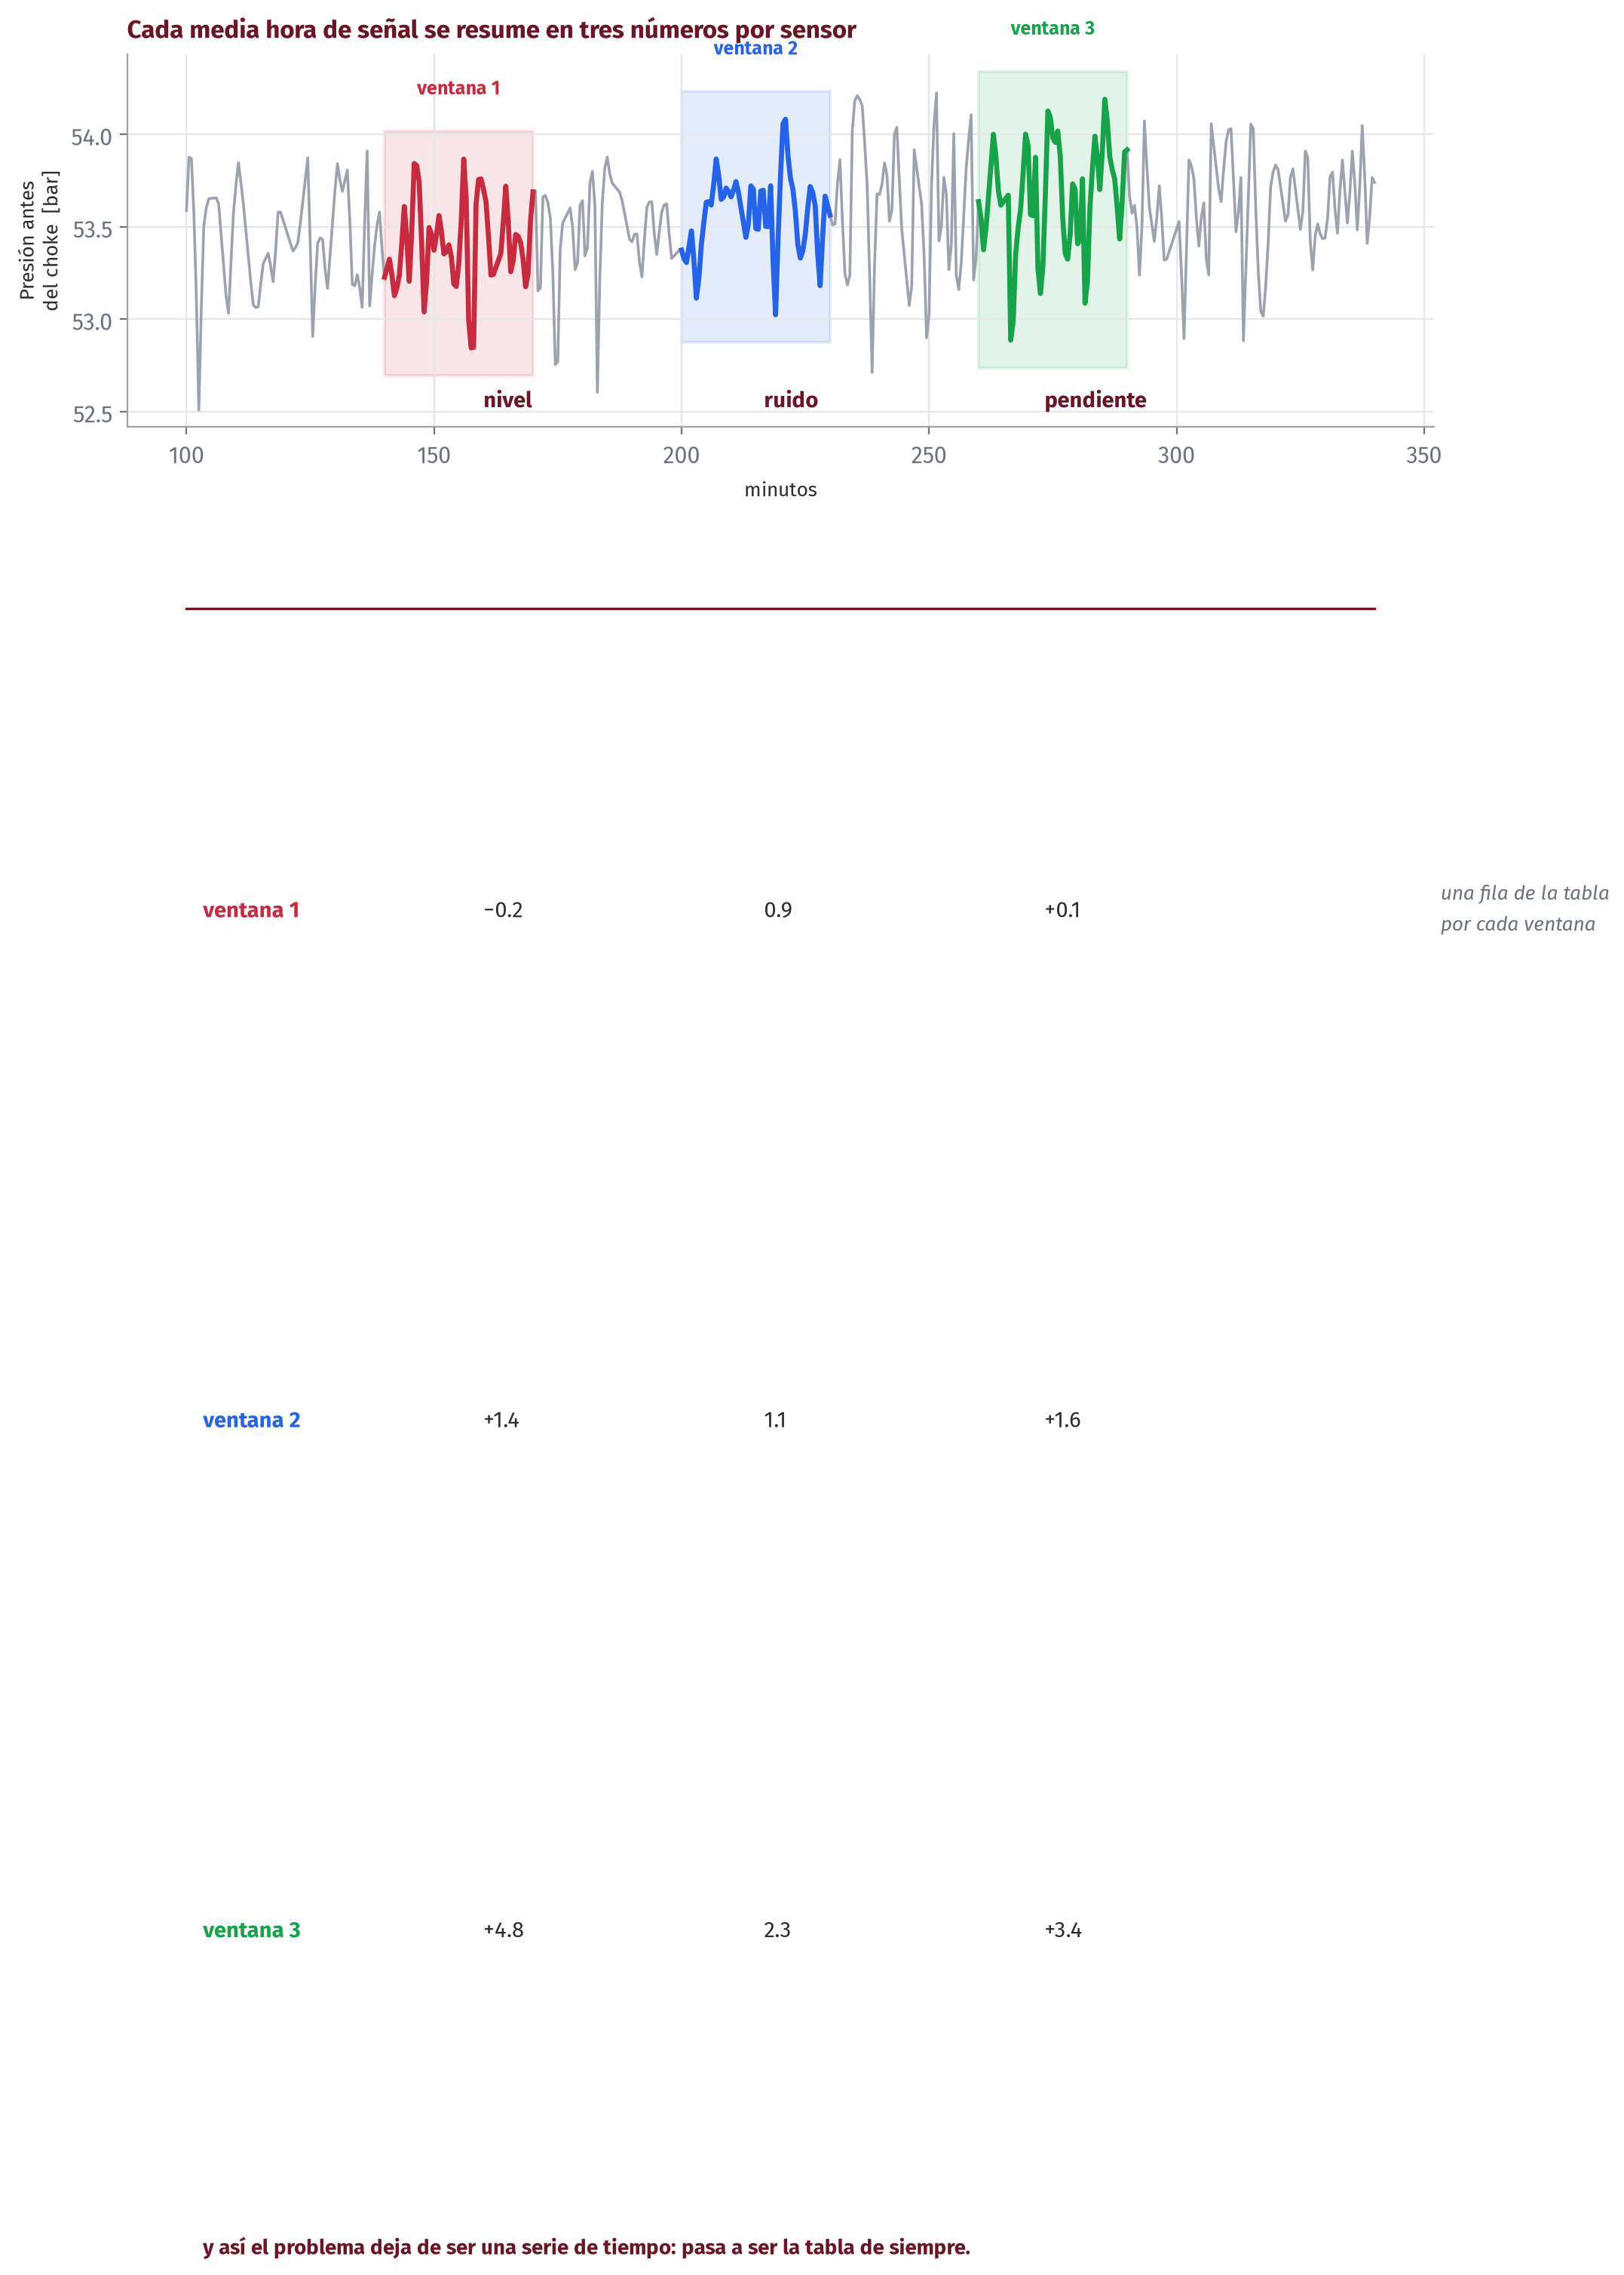
\includegraphics[height=0.80\textheight]{fig_ventana.png}
  \end{center}
\end{frame}

\begin{frame}[shrink=6]{Pero Hay un Problema: Cada Pozo Vive en Otro Mundo}
  \vspace{-6pt}
  \begin{center}
    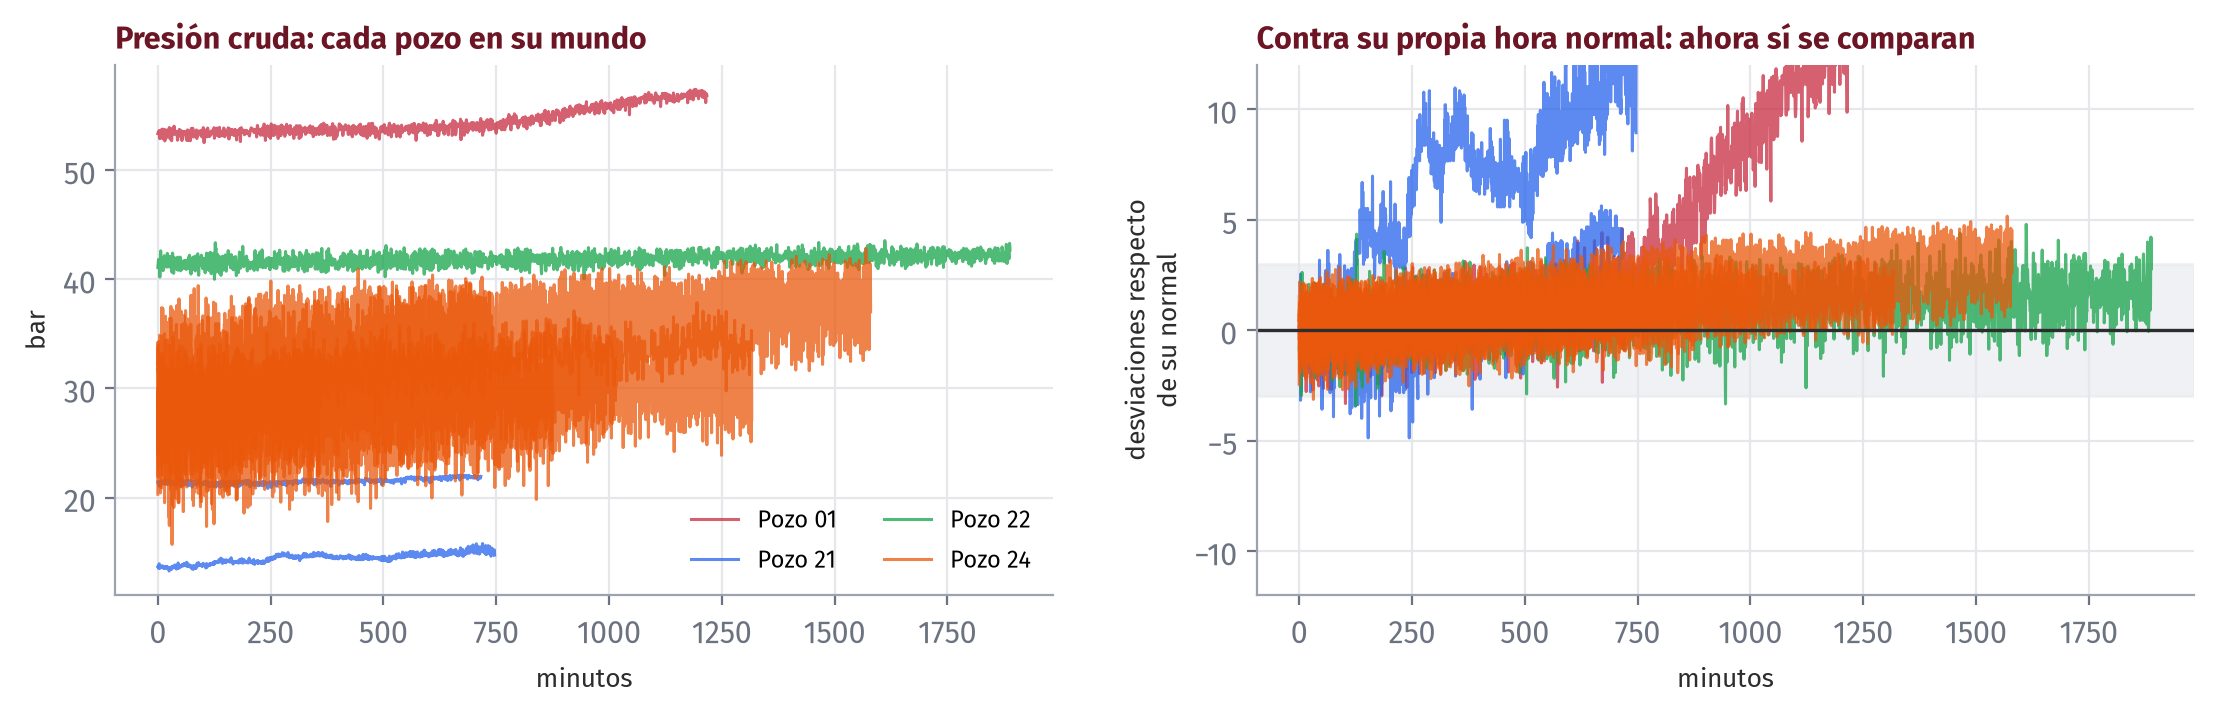
\includegraphics[width=0.98\textwidth]{fig_lineas_base.png}
  \end{center}
  \vspace{-2pt}
  {\footnotesize\color{textMuted}
  \begin{itemize}\setlength{\itemsep}{2pt}
    \item[{\color{arcaRed}\scriptsize\faExclamationTriangle}]
      \textbf{Izquierda:} un pozo trabaja a 54 bar y otro a 130. Si le damos
      esto al modelo, aprende a reconocer \emph{pozos}, no \emph{fallas}.
    \item[{\color{codeGreen}\scriptsize\faCheck}]
      \textbf{Derecha:} las mismas señales, cada una comparada con su propia
      primera hora. Ahora sí hablan el mismo idioma.
  \end{itemize}}
\end{frame}

\begin{frame}[fragile, shrink=20]{La Línea Base: Comparar Cada Pozo Consigo Mismo}
  \vspace{-4pt}
  \begin{columns}[T]
    \begin{column}{0.58\textwidth}
      \begin{pyblock}
def preparar(g):
    """Traduce una grabacion a filas de tabla."""
    X = pd.DataFrame(index=g.index)
    for s in SENSORES:
        v = g[s]

        # 1) su propia normal: la primera hora
        centro = v.iloc[:120].median()
        ancho  = v.iloc[:120].std()

        # 2) la senal en "desviaciones propias"
        z = (v - centro) / ancho
        X[s + "__base"] = z

        # 3) las tres componentes, sobre z
        X[s + "__nivel"] = z.rolling(60).mean()
        X[s + "__ruido"] = z.rolling(60).std()
        X[s + "__pend"]  = z.diff(60)
    return X
      \end{pyblock}
    \end{column}
    \begin{column}{0.40\textwidth}
      \vspace{2pt}
      {\footnotesize\color{textMuted}
      Línea por línea:
      \vspace{4pt}
      \begin{itemize}\setlength{\itemsep}{4pt}
        \item[{\color{arcaRed}\scriptsize\faArrowRight}]
          \texttt{iloc[:120]} $\rightarrow$ las primeras 120 filas,
          o sea la primera hora
        \item[{\color{arcaRed}\scriptsize\faArrowRight}]
          \texttt{median()} $\rightarrow$ el valor típico. Usamos mediana y no
          promedio porque un solo pico no la mueve
        \item[{\color{arcaRed}\scriptsize\faArrowRight}]
          \texttt{rolling(60)} $\rightarrow$ la ventana de 60 filas
          = 30 minutos
        \item[{\color{arcaRed}\scriptsize\faArrowRight}]
          \texttt{diff(60)} $\rightarrow$ cuánto cambió respecto de media
          hora atrás
      \end{itemize}}
      \vspace{5pt}
      {\scriptsize\color{arcaDark}\itshape
        20 columnas: 4 por cada uno de los 5 sensores.}
    \end{column}
  \end{columns}
\end{frame}

% ═════════════════════════════════════════════════════════════════════════════
\sectionframe{El Modelo}{Y la sorpresa: el escalón que más vale no es el algoritmo \\[6pt] \normalsize 82 -- 102 min}
% ═════════════════════════════════════════════════════════════════════════════

\begin{frame}[shrink=8]{Random Forest, Otra Vez y Desde Cero}
  \vspace{-4pt}
  \begin{columns}[T]
    \begin{column}{0.50\textwidth}
      {\small\color{arcaDark}\bfseries\faTree\hspace{5pt}Un árbol de decisión}
      \vspace{4pt}
      {\footnotesize\color{textMuted}
      Es una cadena de preguntas de sí o no, aprendidas del dato:\\[4pt]
      \textit{¿el nivel de temperatura bajó más de 1{,}2? \\
      $\rightarrow$ sí: ¿y el de presión subió más de 0{,}8? \\
      $\rightarrow$ sí: esto es una falla.}\\[5pt]
      Un solo árbol es frágil: cambia un dato y cambia todo.}
    \end{column}
    \begin{column}{0.46\textwidth}
      {\small\color{arcaDark}\bfseries\faUsers\hspace{5pt}Un bosque}
      \vspace{4pt}
      {\footnotesize\color{textMuted}
      Se entrenan \textbf{300 árboles}, cada uno viendo una porción distinta
      de los datos y de las columnas. Después \textbf{votan}.\\[5pt]
      Cada árbol se equivoca por su lado; el promedio de los 300 se equivoca
      mucho menos. Es la sabiduría de la multitud, con árboles.}
    \end{column}
  \end{columns}
  \vspace{8pt}
  \begin{tcolorbox}[colback=arcaGray, colframe=codeGreen, boxrule=0pt, leftrule=3pt,
    arc=3pt, left=8pt, right=8pt, top=5pt, bottom=5pt]
    {\scriptsize\color{codeGreen}\bfseries\faCheck\hspace{4pt}POR QUÉ ESTE Y NO OTRO}\\[4pt]
    {\scriptsize\color{textMuted}
     Porque no le importan las escalas, aguanta columnas inútiles sin
     despeinarse, y --- lo que más nos sirve hoy --- \textbf{nos puede decir
     en qué columnas se apoyó}. Vamos a usar eso para hacerle una pregunta
     de física.}
  \end{tcolorbox}
\end{frame}

\begin{frame}[shrink=8]{Validar con un Pozo que el Modelo Nunca Vio}
  \vspace{-4pt}
  \begin{columns}[T]
    \begin{column}{0.48\textwidth}
      \begin{tcolorbox}[colback=arcaGray, colframe=arcaRed, boxrule=0pt, leftrule=3pt,
        arc=3pt, left=6pt, right=6pt, top=5pt, bottom=5pt]
        {\scriptsize\color{arcaRed}\bfseries\faBan\hspace{4pt}ASÍ NO}\\[4pt]
        {\scriptsize\color{textMuted}
         Mezclar todas las filas y apartar el 20\,\% al azar.\\[4pt]
         Cada pozo quedaría a los dos lados: el modelo ya vio ese pozo, ya
         sabe cómo respira, y en el examen lo reconoce. El número sale
         hermoso y \textbf{es mentira}.}
      \end{tcolorbox}
    \end{column}
    \begin{column}{0.48\textwidth}
      \begin{tcolorbox}[colback=arcaGray, colframe=codeGreen, boxrule=0pt, leftrule=3pt,
        arc=3pt, left=6pt, right=6pt, top=5pt, bottom=5pt]
        {\scriptsize\color{codeGreen}\bfseries\faCheck\hspace{4pt}ASÍ SÍ}\\[4pt]
        {\scriptsize\color{textMuted}
         Sacar \textbf{un pozo entero} y entrenar con los otros tres.
         Después preguntarle por el pozo que nunca vio. Y repetir, dejando
         afuera cada pozo por turno.\\[4pt]
         Eso es \texttt{GroupKFold}, agrupando \textbf{por pozo}.}
      \end{tcolorbox}
    \end{column}
  \end{columns}
  \vspace{8pt}
  {\footnotesize\color{arcaDark}
   La pregunta que responde la forma honesta es la del negocio:
   \textbf{«mañana instalamos esto en un pozo nuevo. ¿Va a funcionar?»}}
  \vspace{6pt}

  {\scriptsize\color{textMuted}\itshape
   Todos los números que siguen salen de esta validación. Ninguno se midió
   sobre datos que el modelo hubiera visto antes.}
\end{frame}

\begin{frame}[shrink=6]{Cada Escalón Hay que Ganárselo}
  \vspace{-8pt}
  \begin{center}
    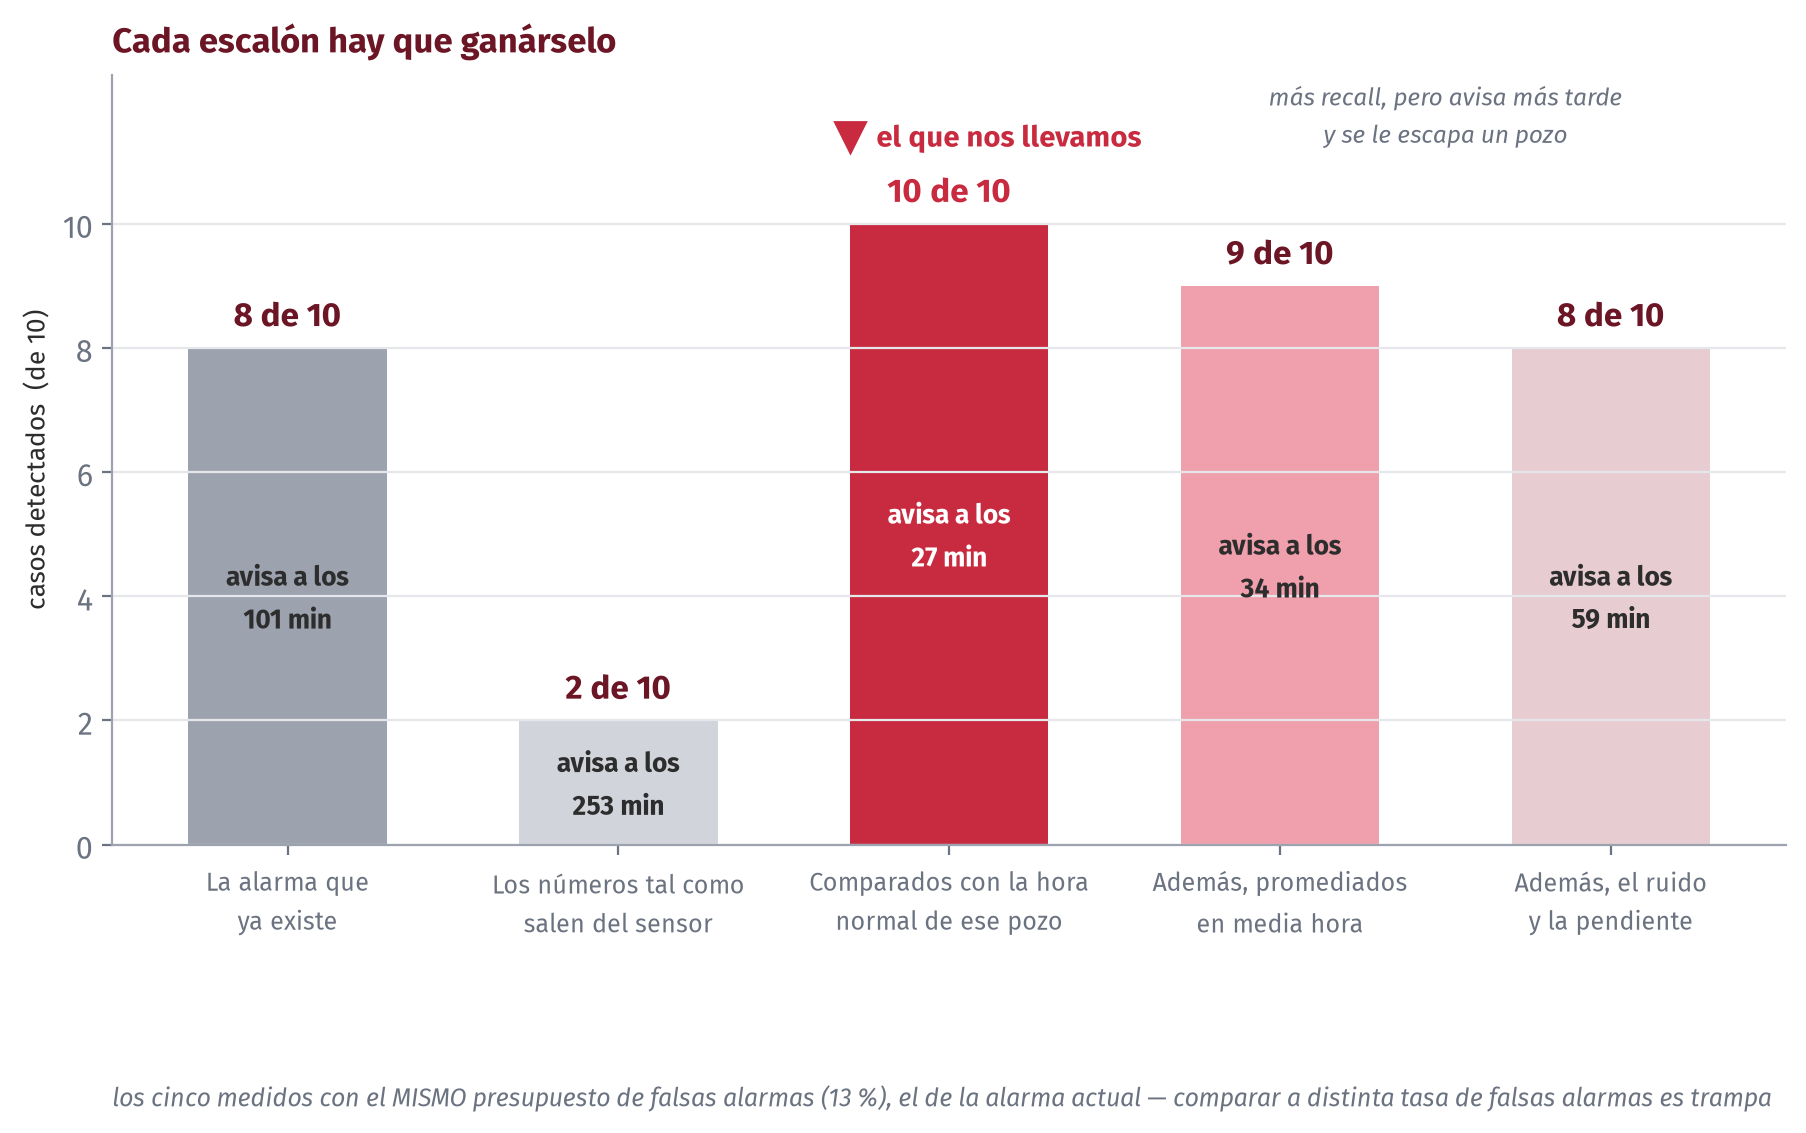
\includegraphics[height=0.80\textheight]{fig_escalera.png}
  \end{center}
\end{frame}

\begin{frame}[shrink=8]{Lo que Dice la Escalera, Leído Despacio}
  \vspace{-4pt}
  {\scriptsize
  \renewcommand{\arraystretch}{1.3}
  \begin{tabular}{@{}p{5.2cm}p{1.8cm}p{1.7cm}p{5.6cm}@{}}
    \toprule
    {\color{arcaDark}\bfseries qué se le dio al modelo} &
    {\color{arcaDark}\bfseries detecta} &
    {\color{arcaDark}\bfseries avisa a los} &
    {\color{arcaDark}\bfseries qué aprendimos} \\
    \midrule
    La alarma que ya existe & 8 de 10 & 101 min & el récord \\
    Los números crudos & {\color{arcaRed}\bfseries 2 de 10} & 253 min &
      {\color{arcaRed}peor que la alarma}: aprende pozos, no fallas \\
    \rowcolor{arcaGray}
    Comparados con su propia normal &
      {\color{arcaRed}\bfseries 10 de 10} & {\color{arcaRed}\bfseries 27 min} &
      {\color{arcaDark}\bfseries el salto. Y no lo dio el algoritmo} \\
    Además, promediados & 9 de 10 & 34 min &
      más estable, pero más tarde \\
    Además, ruido y pendiente & 8 de 10 & 59 min & no aportó \\
    \bottomrule
  \end{tabular}}
  \vspace{9pt}

  \begin{tcolorbox}[colback=arcaGray, colframe=arcaRed, boxrule=0pt, leftrule=3pt,
    arc=3pt, left=8pt, right=8pt, top=6pt, bottom=6pt]
    {\small\color{arcaRed}\bfseries\faStar\hspace{5pt}EL NÚMERO DEL DÍA}\\[5pt]
    {\footnotesize\color{textMuted}
     Entre la fila 2 y la fila 3 hay \textbf{dos líneas de código}: restar la
     mediana y dividir por la desviación. Pasó de \textbf{2 de 10} a
     \textbf{10 de 10}, con el mismo modelo y los mismos datos.}
  \end{tcolorbox}
\end{frame}

\begin{frame}[shrink=6]{Cuánto Tarda Cada Uno en Darse Cuenta}
  \vspace{-8pt}
  \begin{center}
    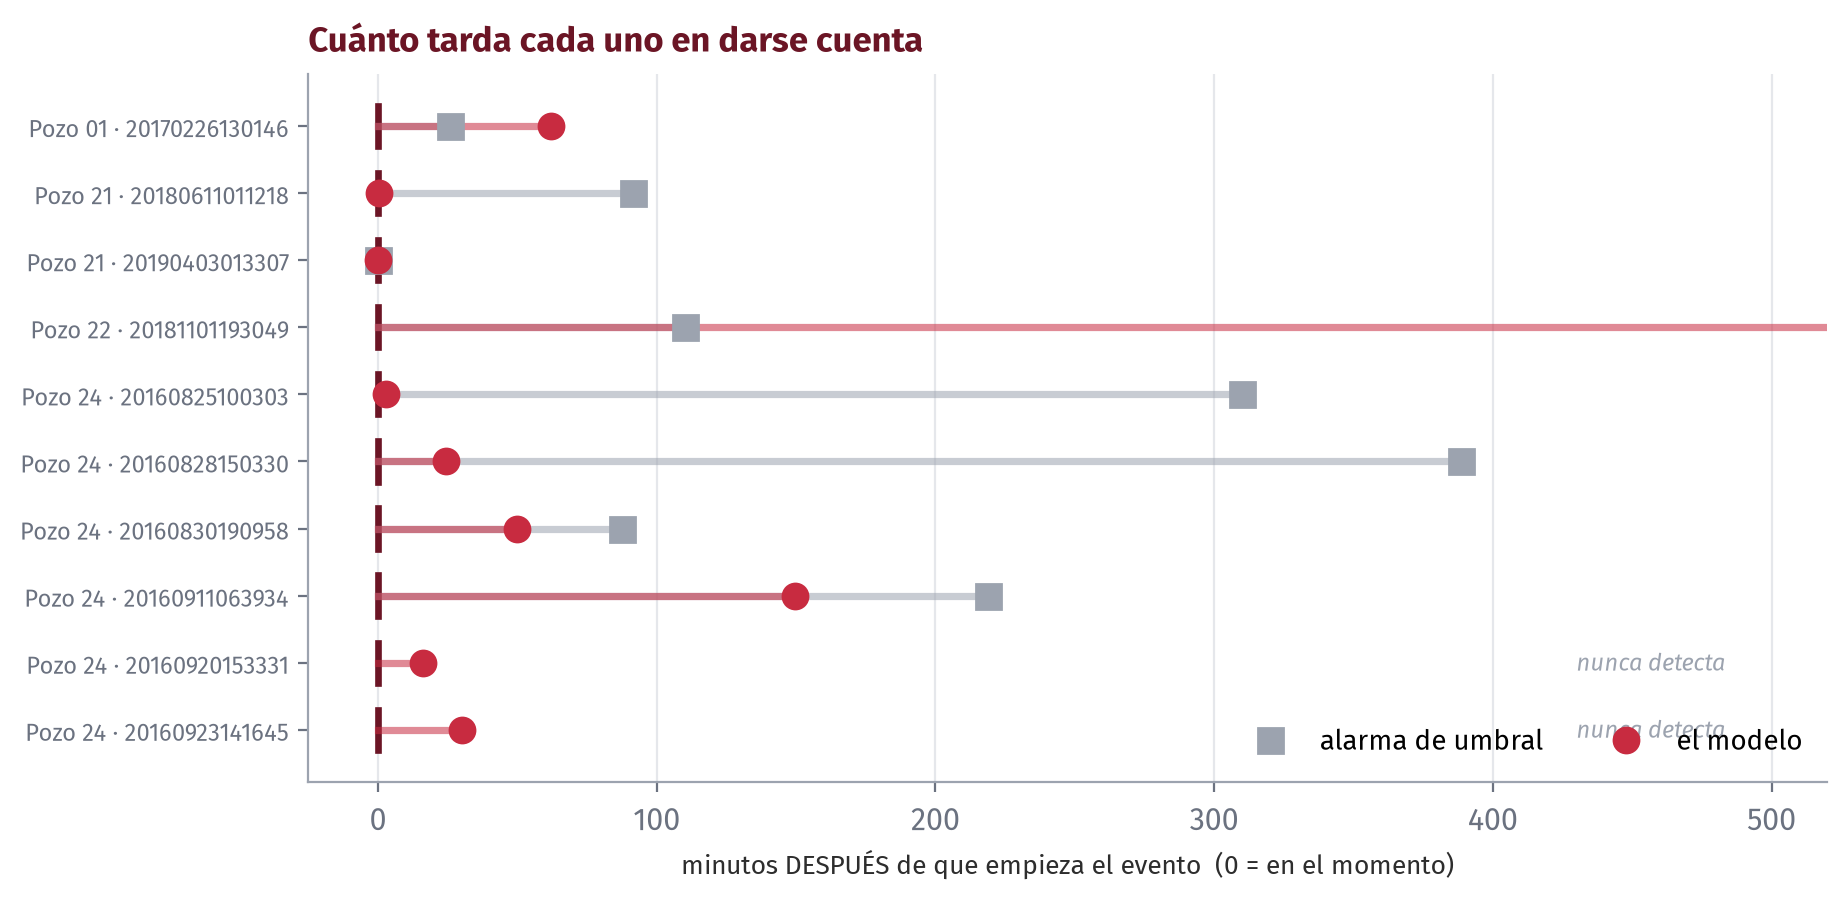
\includegraphics[height=0.72\textheight]{fig_resultado.png}
  \end{center}
  \vspace{-4pt}
  {\footnotesize\color{arcaDark}
   Diez grabaciones, una por línea. La alarma deja \textbf{dos pozos sin
   detectar}; el modelo no deja ninguno.}
\end{frame}

\begin{frame}[shrink=8]{Quién Delata la Incrustación}
  \vspace{-4pt}
  \begin{columns}[T]
    \begin{column}{0.60\textwidth}
      \vspace{-2pt}
      
\includegraphics[width=\textwidth]{fig_importancia.png}
    \end{column}
    \begin{column}{0.37\textwidth}
      {\footnotesize\color{textMuted}
      Le preguntamos al bosque en qué se apoyó. La respuesta \textbf{no es la
      presión}: es la \textbf{temperatura}.
      \vspace{6pt}
      \begin{itemize}\setlength{\itemsep}{4pt}
        \item[{\color{arcaRed}\scriptsize\faArrowRight}]
          La presión sube, sí --- pero también sube cuando alguien cierra
          un poco el choke a propósito.
        \item[{\color{codeGreen}\scriptsize\faCheck}]
          La temperatura aguas abajo \textbf{cayendo mientras la presión
          sube} es la firma de una restricción que \emph{nadie ordenó}.
      \end{itemize}}
      \vspace{6pt}
      {\scriptsize\color{arcaDark}\itshape
        El modelo redescubrió solo el efecto Joule--Thomson.
        Y de paso nos dice qué sensor no hay que dejar sin mantenimiento.}
    \end{column}
  \end{columns}
\end{frame}

\begin{frame}[shrink=6]{No Hay «Un Modelo»: Hay una Perilla}
  \vspace{-6pt}
  \begin{columns}[T]
    \begin{column}{0.58\textwidth}
      \vspace{-4pt}
      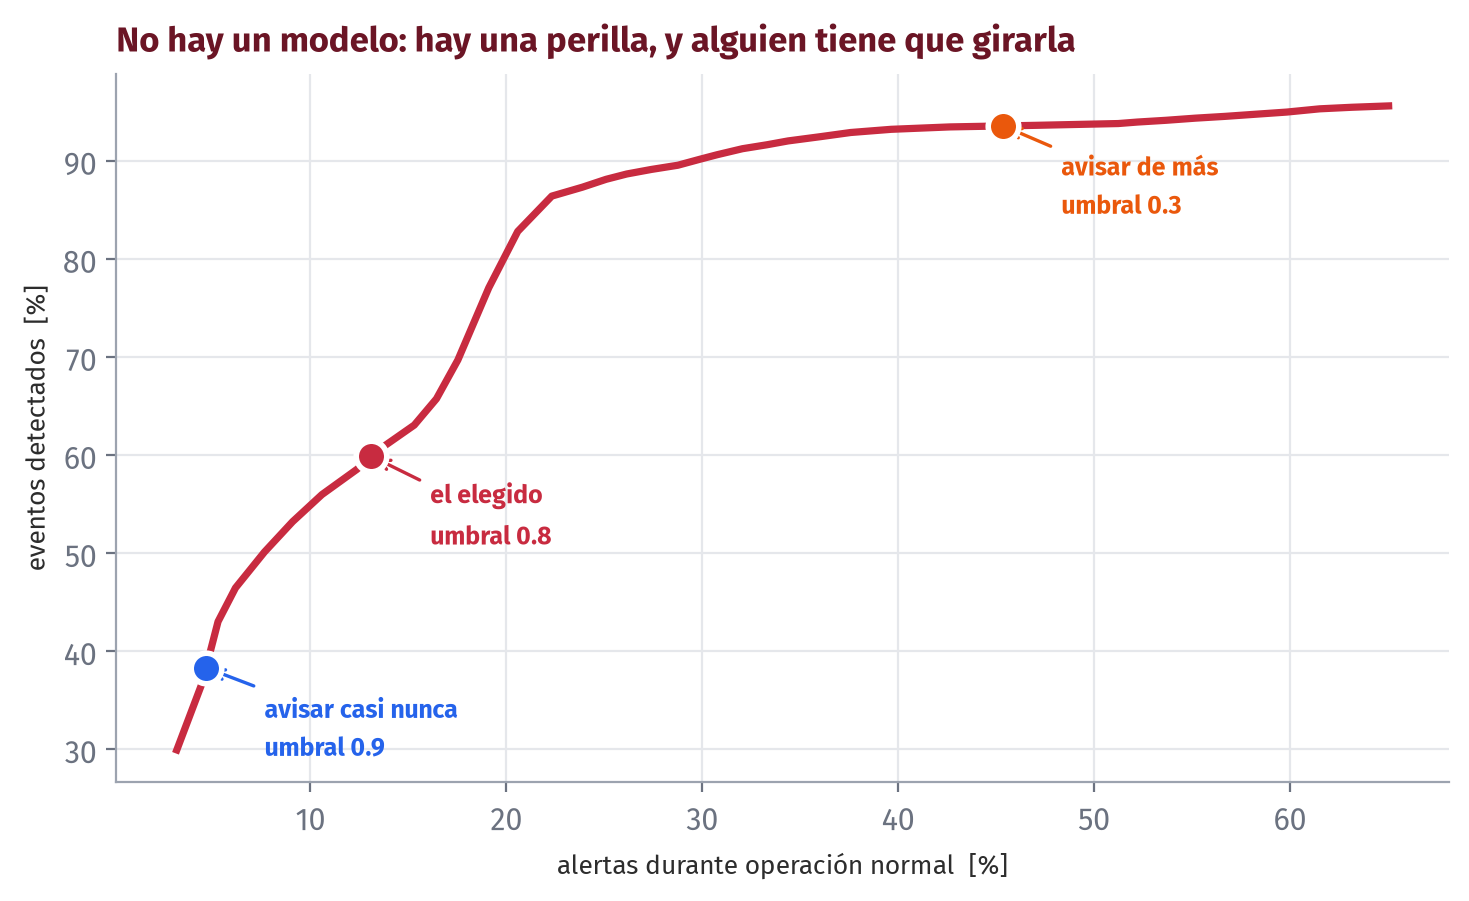
\includegraphics[width=\textwidth]{fig_operacion.png}
    \end{column}
    \begin{column}{0.39\textwidth}
      {\footnotesize\color{textMuted}
      El modelo no dice «sí» o «no»: dice \textbf{qué tan seguro está},
      de 0 a 1. Nosotros elegimos a partir de qué número suena.
      \vspace{6pt}
      \begin{itemize}\setlength{\itemsep}{4pt}
        \item[{\color{codeOrange}\scriptsize\faVolumeUp}]
          Girar hacia \textbf{avisar de más}: no se escapa nada, pero la sala
          de control termina ignorando la pantalla.
        \item[{\color{codeBlue}\scriptsize\faVolumeMute}]
          Girar hacia \textbf{avisar poco}: cada alerta se toma en serio,
          pero algunas fallas pasan.
      \end{itemize}}
      \vspace{6pt}
      \begin{tcolorbox}[colback=arcaGray, colframe=arcaRed, boxrule=0pt, leftrule=3pt,
        arc=3pt, left=6pt, right=6pt, top=4pt, bottom=4pt]
        {\scriptsize\color{textMuted}
         Esa perilla \textbf{no la gira el modelo ni el que programa}.
         La gira quien va a atender la alerta a las tres de la mañana.}
      \end{tcolorbox}
    \end{column}
  \end{columns}
\end{frame}

\begin{frame}[shrink=8]{Cómo Reportarlo al que Decide}
  \vspace{-4pt}
  \begin{columns}[T]
    \begin{column}{0.48\textwidth}
      \begin{tcolorbox}[colback=arcaGray, colframe=arcaRed, boxrule=0pt, leftrule=3pt,
        arc=3pt, left=6pt, right=6pt, top=5pt, bottom=5pt]
        {\scriptsize\color{arcaRed}\bfseries\faBan\hspace{4pt}ASÍ NO}\\[5pt]
        {\scriptsize\color{textMuted}\itshape
         «Entrenamos un Random Forest de 300 árboles con validación
         \texttt{GroupKFold} y obtuvimos un recall de 0{,}605 con un
         \texttt{F1} de 0{,}71.»}\\[5pt]
        {\scriptsize\color{textMuted}
         El gerente no sabe si eso es bueno, no sabe qué hacer mañana,
         y no puede repetirlo en su reunión.}
      \end{tcolorbox}
    \end{column}
    \begin{column}{0.48\textwidth}
      \begin{tcolorbox}[colback=arcaGray, colframe=codeGreen, boxrule=0pt, leftrule=3pt,
        arc=3pt, left=6pt, right=6pt, top=5pt, bottom=5pt]
        {\scriptsize\color{codeGreen}\bfseries\faCheck\hspace{4pt}ASÍ SÍ}\\[5pt]
        {\scriptsize\color{textMuted}\itshape
         «Con los mismos sensores y sin gastar un peso en hardware, pasamos
         de detectar 8 de cada 10 incrustaciones a detectar las 10, y el
         aviso llega \textbf{74 minutos antes}. Sin aumentar las falsas
         alarmas.\\[4pt]
         Eso es una hora y cuarto más para abrir el choke antes de que el
         pozo se cierre solo.»}
      \end{tcolorbox}
    \end{column}
  \end{columns}
  \vspace{8pt}
  {\footnotesize\color{arcaDark}\itshape
   La diferencia no es de estilo. La versión de la derecha se puede
   \textbf{decidir}: dice qué cambia, cuánto cuesta y qué habilita.}
\end{frame}

\begin{frame}[shrink=6]{Las Falsas Alarmas que No lo Eran}
  \vspace{-6pt}
  \begin{center}
    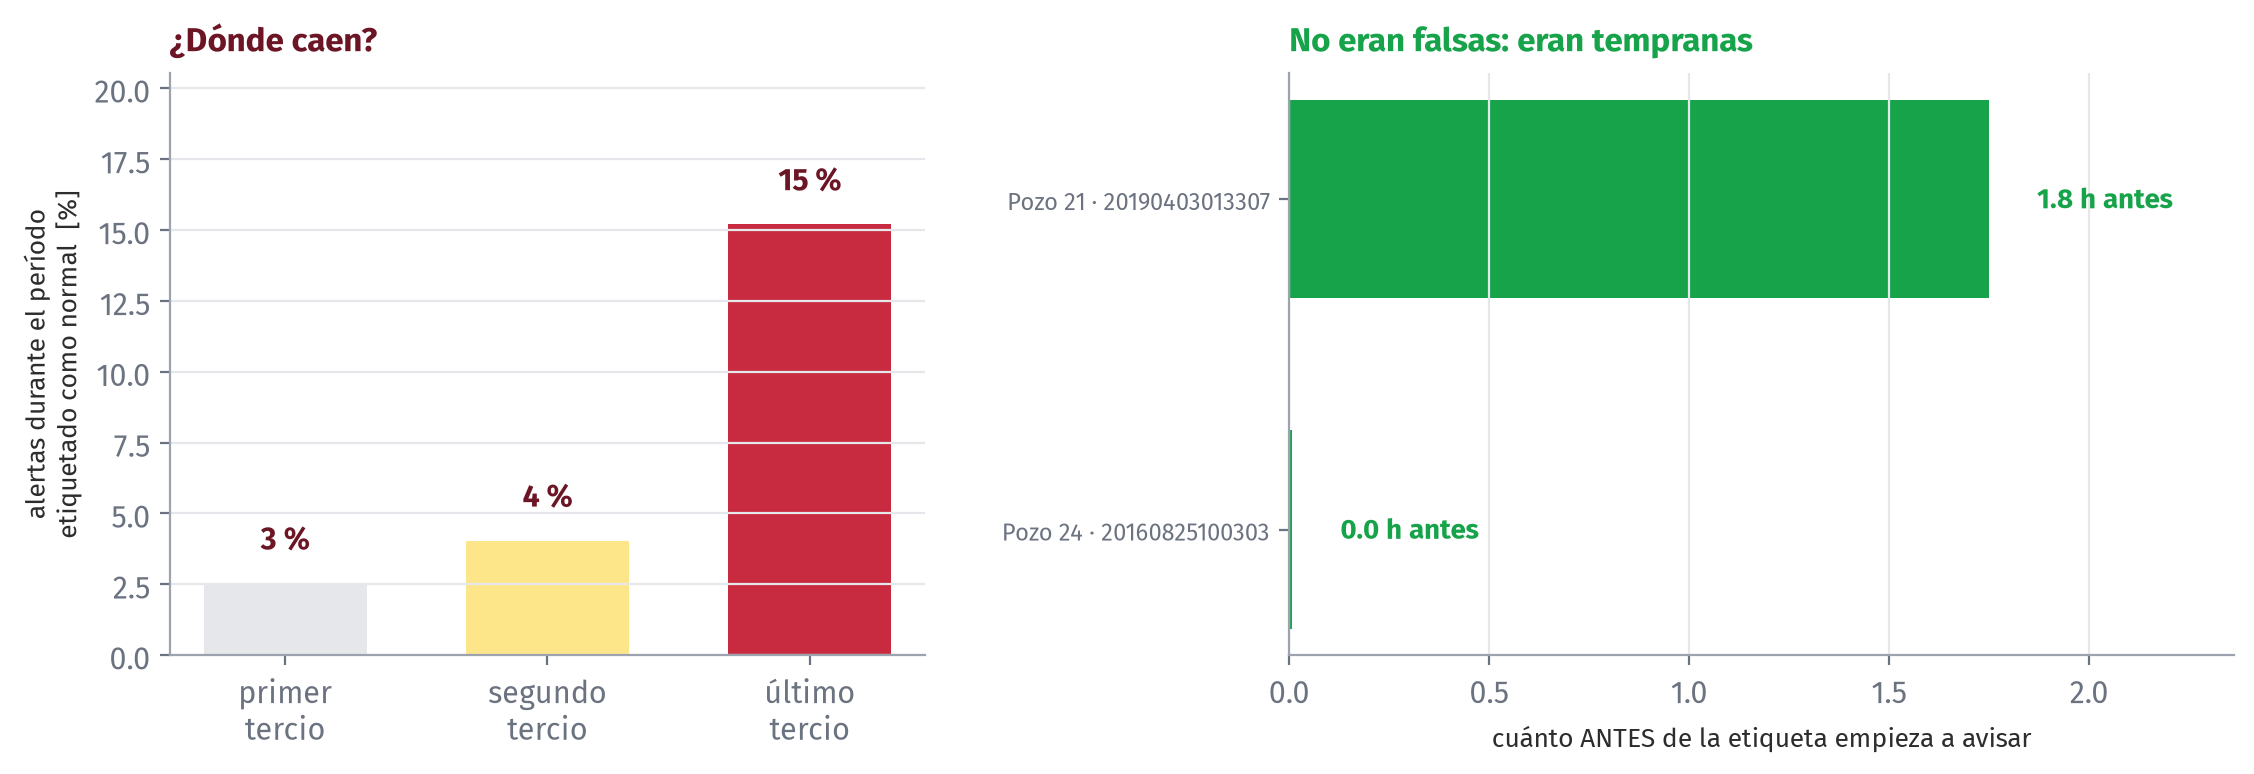
\includegraphics[height=0.66\textheight]{fig_falsas.png}
  \end{center}
  \vspace{-4pt}
  {\footnotesize\color{textMuted}
   Si el modelo se equivocara al azar, las alertas del período normal
   estarían repartidas parejo. \textbf{No lo están}: se amontonan al final,
   justo antes de que el especialista marque el inicio.}
\end{frame}

\begin{frame}[shrink=8]{La Etiqueta No Era la Verdad}
  \vspace{-4pt}
  {\small\color{arcaDark}\bfseries
   Volvamos a la lámina que les pedí anotar al principio.}
  \vspace{8pt}
  \begin{columns}[T]
    \begin{column}{0.50\textwidth}
      {\footnotesize\color{textMuted}
      \begin{itemize}\setlength{\itemsep}{5pt}
        \item[{\color{arcaRed}\scriptsize\faArrowRight}]
          La incrustación \textbf{no empieza en un segundo}: empieza de a poco.
        \item[{\color{arcaRed}\scriptsize\faArrowRight}]
          El especialista tuvo que \textbf{elegir un segundo} para marcar el
          comienzo. Eligió el momento en que a él se le hizo evidente.
        \item[{\color{codeGreen}\scriptsize\faCheck}]
          Cuando el modelo avisa antes de esa marca, la métrica lo cuenta
          como \textbf{error}. En un pozo, ese «error» llegó
          \textbf{1 hora y 48 minutos antes}.
      \end{itemize}}
    \end{column}
    \begin{column}{0.46\textwidth}
      \begin{tcolorbox}[colback=arcaGray, colframe=arcaDark, boxrule=0pt, leftrule=3pt,
        arc=3pt, left=6pt, right=6pt, top=6pt, bottom=6pt]
        {\scriptsize\color{arcaDark}\bfseries\faLightbulb[regular]\hspace{4pt}LA LECCIÓN INCÓMODA}\\[5pt]
        {\scriptsize\color{textMuted}
         Una métrica compara al modelo contra la etiqueta, no contra la
         realidad.\\[5pt]
         Si la etiqueta es el juicio de una persona, entonces
         \textbf{«equivocarse» puede significar acertar antes que ella}.\\[5pt]
         Por eso ningún resultado se cierra sin ir a mirar
         \textbf{dónde} se equivoca.}
      \end{tcolorbox}
    \end{column}
  \end{columns}
\end{frame}

% ═════════════════════════════════════════════════════════════════════════════
\sectionframe{Su Turno}{El pozo que dejamos afuera \\[6pt] \normalsize 102 -- 118 min}
% ═════════════════════════════════════════════════════════════════════════════

\begin{frame}[shrink=8]{Su Turno: el Pozo con Dos Sensores \hfill {\normalsize\color{arcaRed}\faClock\hspace{4pt}18 min}}
  \vspace{-4pt}
  \begin{tcolorbox}[colback=arcaGray, colframe=arcaDark, boxrule=0pt, leftrule=3pt,
    arc=3pt, left=8pt, right=8pt, top=5pt, bottom=5pt]
    {\footnotesize\color{arcaDark}\itshape
     El \textbf{pozo 23} tiene 141 horas grabadas y solo \textbf{dos}
     sensores vivos. Es el pozo más real de todos: así llegan los datos
     cuando nadie los preparó para una clase.}
  \end{tcolorbox}
  \vspace{7pt}
  {\footnotesize\color{textMuted}
  \begin{enumerate}\setlength{\itemsep}{4pt}
    \item Corran la celda que ya está escrita: arma la tabla del pozo 23 con
          los dos sensores que sí tiene. \textbf{El primer paso ya está resuelto.}
    \item Entrenen con los cuatro pozos de la clase y pregúntenle por el 23.
          ¿Cuántos de sus \textbf{dos} eventos detecta? ¿A los cuántos minutos?
    \item Giren la perilla. Busquen el umbral que detecta los dos eventos.
          ¿Cuántas falsas alarmas costó?
    \item Comparen contra la alarma de umbral sobre el mismo pozo.
          ¿Gana el modelo con solo dos sensores?
    \item {\color{arcaDark}\bfseries Pregunta de negocio:} escriban
          \textbf{una frase} para el jefe de operaciones que responda:
          \textit{¿instalamos esto en el pozo 23, o primero arreglamos los
          tres sensores muertos?} La frase tiene que decir qué se gana
          con cada opción.
  \end{enumerate}}
\end{frame}

% ═════════════════════════════════════════════════════════════════════════════
\sectionframe{Cierre}{}
% ═════════════════════════════════════════════════════════════════════════════

\begin{frame}[shrink=10]{Lo Que Aprendimos Hoy}
  \vspace{-4pt}
  \begin{columns}[T]
    \begin{column}{0.48\textwidth}
      {\small\color{arcaDark}\bfseries\faLightbulb[regular]\hspace{5pt}Conceptos:}
      \vspace{4pt}
      {\footnotesize\color{textMuted}
      \begin{itemize}\setlength{\itemsep}{3pt}
        \item[{\color{codeGreen}\scriptsize\faCheck}]
          Toda señal es \textbf{nivel + lo que se repite + ruido}
        \item[{\color{codeGreen}\scriptsize\faCheck}]
          Una \textbf{ventana deslizante} convierte una señal en una tabla
        \item[{\color{codeGreen}\scriptsize\faCheck}]
          Comparar cada activo \textbf{consigo mismo} antes de comparar
          entre activos
        \item[{\color{codeGreen}\scriptsize\faCheck}]
          Validar dejando \textbf{una unidad entera por fuera}
        \item[{\color{codeGreen}\scriptsize\faCheck}]
          Una \textbf{etiqueta} es un juicio humano, no la verdad
      \end{itemize}}
    \end{column}
    \begin{column}{0.48\textwidth}
      {\small\color{arcaDark}\bfseries\faTools\hspace{5pt}Herramientas:}
      \vspace{4pt}
      {\footnotesize\color{textMuted}
      \begin{itemize}\setlength{\itemsep}{3pt}
        \item[{\color{arcaRed}\scriptsize\faArrowRight}]
          \texttt{.rolling(n).mean()} \textbf{.std()} \texttt{.diff(n)}
        \item[{\color{arcaRed}\scriptsize\faArrowRight}]
          \texttt{RandomForestClassifier}
        \item[{\color{arcaRed}\scriptsize\faArrowRight}]
          \texttt{GroupKFold(groups=pozo)}
        \item[{\color{arcaRed}\scriptsize\faArrowRight}]
          \texttt{predict\_proba} y el \textbf{umbral} como decisión
      \end{itemize}}
      \vspace{6pt}
      \begin{tcolorbox}[colback=arcaGray, colframe=arcaRed, boxrule=0pt, leftrule=3pt,
        arc=3pt, left=6pt, right=6pt, top=4pt, bottom=4pt]
        {\scriptsize\color{arcaRed}\bfseries EL NÚMERO DEL DÍA}\\[3pt]
        {\scriptsize\color{textMuted}
         \textbf{74 minutos.} Lo que se ganó sin comprar un solo sensor
         nuevo.}
      \end{tcolorbox}
    \end{column}
  \end{columns}
\end{frame}

\begin{frame}[shrink=8]{Si Se Llevan Una Sola Cosa}
  \vspace{6pt}
  \begin{tcolorbox}[colback=arcaGray, colframe=arcaRed, boxrule=0pt, leftrule=4pt,
    arc=3pt, left=10pt, right=10pt, top=9pt, bottom=9pt]
    {\large\color{arcaDark}\bfseries
     El algoritmo no cambió en toda la clase.}\\[7pt]
    {\footnotesize\color{textMuted}
     El mismo Random Forest pasó de detectar \textbf{2 de 10} a detectar
     \textbf{10 de 10} --- y lo único que cambió fueron dos líneas que
     comparan cada pozo con su propia hora normal.\\[6pt]
     Elegir bien qué se le pregunta al dato valió más que cualquier modelo.
     Y eso no lo hace la librería: lo hace \textbf{alguien que entiende el
     pozo}.}
  \end{tcolorbox}
  \vspace{8pt}
  {\footnotesize\color{arcaDark}\itshape
   Por eso este módulo se llama \emph{Machine Learning aplicado a ingeniería
   de yacimientos y producción}, y no \emph{Machine Learning}.}
\end{frame}

\begin{frame}[shrink=8]{Lo Que Sigue}
  \vspace{4pt}
  {\footnotesize\color{textMuted}
  \begin{itemize}\setlength{\itemsep}{9pt}
    \item[{\color{arcaRed}\faArrowCircleRight}]
      \textbf{Clase 3 --- Curvas de declinación y cuánto queda.}
      Arps (1945), la deuda que dejamos anotada en la Clase 1: exponencial,
      hiperbólica, y el EUR. Ahí vuelve el ciclo estacional que hoy no
      existía, porque el dato va a ser mensual.
    \item[{\color{arcaRed}\faArrowCircleRight}]
      \textbf{Clase 4 --- El agua y el gas como diagnóstico.}
      WOR, GOR y la llegada del agua: cuándo el yacimiento avisa que está
      cambiando.
    \item[{\color{arcaRed}\faArrowCircleRight}]
      \textbf{Clase 5 --- Bombas ESP y levantamiento artificial.}
      El mismo método de hoy, sobre el equipo que más se rompe y más caro
      cuesta reparar.
  \end{itemize}}
  \vspace{8pt}
  {\scriptsize\color{arcaDark}\itshape
   Y una promesa que se paga hoy mismo: en la Clase 1 dijimos que
   íbamos a nombrar la recta sobre el logaritmo. Se llama
   \textbf{declinación exponencial de Arps}, y la completamos en la Clase 3.}
\end{frame}

\begin{frame}[shrink=10]{Datos y Referencias}
  \vspace{4pt}
  {\footnotesize\color{textMuted}
  \begin{itemize}\setlength{\itemsep}{6pt}
    \item[{\color{arcaRed}\scriptsize\faDatabase}]
      \textbf{3W Dataset v2.0.0} --- Petrobras.
      \texttt{github.com/petrobras/3W}\\
      Instancias reales de eventos indeseados en pozos costa afuera.
      Datos bajo licencia \textbf{CC BY 4.0}.
    \item[{\color{arcaRed}\scriptsize\faBook}]
      Vargas, R. E. V. \emph{et al.} (2019). \textit{A realistic and public
      dataset with rare undesirable real events in oil wells}. Journal of
      Petroleum Science and Engineering, 181, 106223.
    \item[{\color{arcaRed}\scriptsize\faFileCode}]
      El subconjunto que usamos hoy se arma con
      \texttt{modulo5-clase2/preparar\_datos.py}, y todas las figuras y
      números de estas láminas salen de \texttt{figuras.py}.
      Nada está escrito a mano.
  \end{itemize}}
  \vspace{8pt}
  {\scriptsize\color{arcaDark}\itshape
   Si quieren repetir cualquier número de hoy: clonan el repositorio,
   corren los dos scripts, y tiene que dar exactamente lo mismo.
   Si no da, es un error nuestro y queremos saberlo.}
\end{frame}

% ── GRACIAS ──────────────────────────────────────────────────────────────────
\begingroup
\setbeamertemplate{headline}{}
\setbeamertemplate{footline}{}
\setbeamertemplate{navigation symbols}{}
\begin{frame}[plain, noframenumbering]
  \begin{tikzpicture}[remember picture, overlay]
    \fill[arcaDark] (current page.south west) rectangle (current page.north east);
    \node[anchor=center, text=white, font=\Huge\bfseries]
      at ([yshift=1.5cm]current page.center) {¡Gracias!};
    \node[anchor=center, text=white!80, font=\large, text width=10cm, align=center]
      at ([yshift=0.2cm]current page.center)
      {Carlos Enrique Mosquera Trujillo};
    \node[anchor=center, text=white!60, font=\normalsize, text width=10cm, align=center]
      at ([yshift=-0.6cm]current page.center)
      {\faEnvelope\hspace{6pt}cmosquerat@unal.edu.co};
    \node[anchor=center, text=white!60, font=\normalsize, text width=11cm, align=center]
      at ([yshift=-1.3cm]current page.center)
      {Machine Learning for Petroleum Engineers Using Python};
    \node[anchor=center, text=white!40, font=\small]
      at ([yshift=-2.0cm]current page.center)
      {Módulo 5 · Clase 2 \quad$\cdot$\quad SLB Ecuador \quad$\cdot$\quad UDLA \quad$\cdot$\quad 2026};
  \end{tikzpicture}
\end{frame}
\endgroup

\end{document}
